\documentclass[10pt,twocolumn,letterpaper]{article}

\usepackage[T1]{fontenc}
\usepackage[utf8]{inputenc}
\usepackage{newtxtext,newtxmath}
\usepackage[letterpaper,top=0.9in,bottom=1in,left=0.85in,right=0.85in,columnsep=0.25in]{geometry}
\usepackage{microtype}
\usepackage{booktabs}
\usepackage{array}
\usepackage{adjustbox}
\usepackage{float}
\usepackage{graphicx}
\usepackage{xcolor}
\usepackage{caption}
\usepackage{subcaption}
\usepackage{enumitem}
\usepackage{amsmath}
\usepackage{tikz}
\usetikzlibrary{positioning,arrows.meta,shapes.misc,fit,calc}
\usepackage[numbers,sort&compress]{natbib}
\usepackage[hyphens]{url}
\usepackage[hidelinks]{hyperref}

\graphicspath{{figures/}}
\raggedbottom
% Let float pages fill up before a new one is opened (packs the appendix tables).
\renewcommand{\topfraction}{0.9}
\renewcommand{\dbltopfraction}{0.9}
\renewcommand{\textfraction}{0.07}
\renewcommand{\floatpagefraction}{0.8}
\renewcommand{\dblfloatpagefraction}{0.8}
\setcounter{topnumber}{4}
\setcounter{dbltopnumber}{4}
\setcounter{totalnumber}{6}
\captionsetup{font=small,labelfont=bf,skip=4pt}
\setlist{nosep,leftmargin=*}
\setlength{\bibsep}{2pt}
\newcommand{\pp}{\,pp}
\newcommand{\qone}{Query~1}
\newcommand{\qtwo}{Query~2}

\title{\Large\bfseries Package Hallucinations Revisited: Measurement Validity, Replication, and Tail Risk in Modern Code Models}
\author{Jacob Anderson\\ \small\texttt{jwa@beyond-ordinary.com}}
\date{\small Manuscript draft, September 2026}

\begin{document}
\maketitle

\begin{abstract}
When a code model recommends a package that does not exist on the registry, anyone can register
that name and fill it with malicious code. Several studies now report how often models do this. We
show that the reported rate depends heavily on how it is measured. We re-ran the 2024 study by
Spracklen et al.\ under its own settings, with three random seeds per model. We built a stricter
parser that refuses to mine package names out of prose or code, and we checked it against labeled
samples. We ran a controlled test of the token cap that earlier work had blamed for large rate
changes. We then measured six current models on the same 800 Python prompts, with two package
questions per prompt, under a plan fixed before any data were collected. Three later cells added
Qwen 3.5, Kimi K2.7, and Kimi K3. The old results mostly hold up. CodeLlama came out at 24.55\%
against a published 26.12\%. DeepSeek kept its rank, but under its own original parser it scored
13.28--13.54\%, below the published 16.61\%, and every seed's confidence interval excluded that
value. The token-cap effect that we and an independent audit had reported earlier
\citep{anderson2026replication,codex2026audit} did not reappear as a consistent or monotone effect.
Modern models ranged from 1.31\% to 17.91\%, but the average hides three different kinds of failure.
For Grok~4.6 and DeepSeek V4 Flash, three answers supplied 82.88\% and 72.42\% of all unregistered
names; DeepSeek Coder V2's 10.30\% was spread across many prompts. Kimi K3 pushed the range to
33.30\%, yet 46 answers that hit the token cap supplied 81.02\% of its unregistered names, and it put
fewer prompts at risk than its predecessor, so the ranking between the two flips with the choice of
metric. Rescoring the same outputs with the extractor of a concurrent 2026 replication kept the
original six cells at 8.30--17.49\%, and four of the five names that all six models produced came
from one identical prompt. A single average rate is not enough. Rates need a dated registry, a stated
parser with its coverage, confidence intervals built on prompts, and a measure of how concentrated
the errors are.
\end{abstract}

\section{Introduction}
\label{sec:intro}

\subsection{Motivation}

Code models do more than write code. Ask one which packages you need, and it answers with names. If
one of those names is not registered on the package index, anyone can register it. This is the
\emph{slopsquatting} threat \citep{nesbitt2025slopsquatting,gooding2025slopsquatting}: an attacker
publishes a malicious package under a name that models are already telling developers to install
\citep{lanyado2023trust,lanyado2024diving,spracklen2025package}. Typosquatting
\citep{neupane2023beyond,ohm2020backstabber,zimmermann2019small,ladisa2023sok} waits for a developer
to mistype a name. Slopsquatting does not have to wait. The model supplies both the name and the
confidence.

Two distinctions matter before we count anything. First, a recommendation is not the same as an
import. An install command, or an answer to ``which packages do I need,'' is an explicit
recommendation. An import statement inside generated code might just refer to a file in the same
project. Second, a name that is not on PyPI is not necessarily made up. Models often name real tools
from other ecosystems, such as \texttt{apt}, npm, Java, or Go packages, that simply cannot be
installed with pip. They also name Python standard-library modules as if they were packages. All of
these are unsafe recommendations, but they are different mistakes. So we measure an
\emph{unregistered-PyPI recommendation rate}, and we use the word ``hallucination'' only for the
older metric that we replicate.

This is also why replication is hard. A reported rate depends on four choices: how the model's free
text is turned into package names, which snapshot of the registry counts as the truth, how many
tokens the model was allowed to produce, and how the errors are spread across answers. None of these
is a small detail. Each of them changed a conclusion in the work reported here.

\subsection{Gap}

Spracklen et al.\ \citep{spracklen2025package} established the problem at scale. Across 16 models
and 576,000 code samples, 19.7\% of recommended packages did not exist, and 205,474 different invented
names appeared. A 2026 replication on five frontier models \citep{churilov2026range} reports that the
gap between models has narrowed and that some names are invented by every model. Both studies report
one average rate per model. Our own first attempt to replicate the 2024 result through a plain HTTP
client \citep{anderson2026replication}, checked by an independent audit \citep{codex2026audit},
found four ways that an average can mislead:
\begin{itemize}
\item A permissive parser that splits text on commas counts code fragments and prose as invented
  packages.
\item A token cap can silently produce empty answers from a reasoning model, or cut a list in the
  middle of a name.
\item The registry changes over time, so a name can switch from ``invented'' to ``real'' with no
  change in the model.
\item A 2024 checkpoint served through a 2026 stack is not provably the same model.
\end{itemize}
An average also cannot tell you whether the risk is spread evenly or concentrated in a few runaway
answers. Those two situations call for different defenses.

\subsection{Contributions}

\begin{enumerate}
\item A properly powered replication of the 2024 result, with three seeds per model, that separates
  ``the pattern holds'' from ``the exact number holds'' (\S\ref{sec:tracka}).
\item A strict, validated parser that refuses unclear answers instead of guessing, checked again on
  the newer hosted-model output formats after the campaign (\S\ref{sec:instrument},
  \S\ref{sec:validation}).
\item A controlled experiment on the token cap, with identical prompts and deterministic decoding
  (\S\ref{sec:cap}).
\item A benchmark of six current models on the same prompts, scored against two registry snapshots,
  with confidence intervals that respect the prompt structure and a way to tell diffuse failures from
  catastrophic ones (\S\ref{sec:trackb}--\S\ref{sec:pairwise}). Three later cells extend it, and the
  comparison between Kimi K2.7 and Kimi K3 shows a ranking that flips with the choice of metric
  (\S\ref{sec:extension}, \S\ref{sec:k3}).
\item A direct comparison with the concurrent Churilov study, made by rescoring our own outputs
  with that study's extractor, plus an overlap analysis that asks whether names shared across models
  come from shared prompts (\S\ref{sec:bridge}).
\end{enumerate}

\subsection{Result preview}

\begin{itemize}
\item CodeLlama 7B: 24.55\% (mean of three seeds) against a published 26.12\%.
\item DeepSeek Coder 6.7B under its original parser: 13.43\% against a published 16.61\%. All three
  seed intervals exclude the published value.
\item Token cap: no consistent or monotone effect in the controlled test.
\item Modern models: primary rates from 1.31\% to 17.91\%, with very different concentration.
\item Rescoring with Churilov's extractor: the original six Campaign~4 cells stay at 8.30--17.49\%.
  The extension cells score 6.51\% (Qwen 3.5), 7.38\% (Kimi K2.7), and 8.37\% (Kimi K3). Of the 621
  flagged mentions, 608 (97.91\%) come from imports rather than install commands.
\item Overlap: five names appear in all six Campaign~4 models, and four of them appear in all six on
  the same prompt.
\item Cloud extension: Qwen 3.5 at 2.77\% (95\% interval 2.07--3.54). Kimi K2.7 at 23.10\%, but only
  4.95\% among answers with at most ten packages, and rising steeply with list position.
\item Kimi K3: 33.30\% (27.22--38.81) when every recommended name counts equally, 21.50\% of prompts
  at risk, and a 4.18\% mean rate per answer. Setting aside its 46 cap-hit answers, as a diagnostic
  only, gives 13.11\%, next to K2.7's 13.18\%.
\end{itemize}

\section{Background and related work}
\label{sec:background}

\subsection{Package hallucinations and supply-chain risk}

The original study \citep{spracklen2025package} counts package hallucinations in three ways. It
parses \texttt{pip install} and \texttt{npm install} commands out of generated code. It asks the
model which packages its own generated code requires. And it asks the model which packages would be
useful for the original task. Every extracted name is normalized and looked up in a master list of
registry names taken on 2024-01-10. Any name that is missing from the list counts as a hallucination.
The threat model is an attacker with no special access who can register packages. The study withheld
the hallucinated names themselves for safety. We adopt both the threat model and the release policy:
no candidate unregistered name appears in this paper or its artifacts. The original study describes
the threat as a variation of the classical package confusion attack. The name
\emph{slopsquatting}, modeled on typosquatting, was coined by Seth Larson and popularized by Andrew
Nesbitt in April 2025 \citep{nesbitt2025slopsquatting,gooding2025slopsquatting}, roughly ten months
after the study's preprint appeared.

Three terms recur below. A \emph{package recommendation} is a name the model offered when asked a
package question. A \emph{generated import} is a name that appears in an import statement of
generated code. An \emph{unregistered name} is absent from the relevant PyPI snapshot, and an
\emph{ecosystem mismatch} is an unregistered name that is a real package somewhere else. All of these
matter for slopsquatting, but only rates built on the same channel can be compared across studies.

\subsection{Evaluation of code-generating models}

Code benchmarks \citep{chen2021codex} pin a model version and report one number per model. Hosted
models make pinning harder, because the same alias can serve a different model next month. Decoding
is random, so one run is one draw, and two models should be compared on the same prompts, pair by
pair. Most important for this measurement, the package names in one answer are not independent
observations. They share a prompt, a task, and a single generation. Treating each name as its own
coin flip is pseudoreplication \citep{hurlbert1984pseudoreplication}. The right unit for resampling is
the cluster, here the prompt \citep{cameron2008bootstrap,efron1993bootstrap}.

\subsection{Measurement error in free-form generations}

Turning free text into package names is a classification task, and it has its own precision and
recall. A permissive parser catches almost everything but invents false positives whenever the model
stops following the requested format. A strict parser refuses answers that do not follow the format
and misses real recommendations buried in prose. Either way, the choice is part of the measurement
and belongs next to the rate. Registry membership also changes over time. Names get registered and
deleted after any snapshot, so a name can move from ``hallucinated'' to real, or from real to
deleted, while the model stays the same. Finally, the shape of the response matters. A token cap cuts
lists short. A reasoning model can spend its whole budget on hidden reasoning and return nothing. A
hosted endpoint can leak a literal control token into the text. Each of these looks like model
behavior if nobody checks.

\subsection{Concurrent 2026 replication}

Churilov \citep{churilov2026range} re-ran the full original prompt corpus (199,845 Python and
JavaScript generations) on five frontier models released between October 2025 and March 2026. That
study extracts package references from generated code (install commands plus imports) and checks
them against the original master lists. Beyond the replication, it finds 127 names that all five
models invent, of which 53 could still be registered after coordinated disclosure with PyPI Security
and Socket.dev. It also reports that Python now has a higher rate than JavaScript, and that Claude
Haiku 4.5 scores below Claude Sonnet 4.6. It is the broader study in languages, corpus size,
registrability testing, and disclosure, and it shows that the cross-model attack surface is real.

Three points matter for the comparison in \S\ref{sec:bridge}. First, its code-import measure is not
the original study's three-channel measure, and it is not our package-recommendation measure either.
A rate from one is not a rate from the other. Second, its headline that the range between models has
compressed (4.62--6.10\% overall, 5.49--7.27\% on Python, against 5.2\% and 21.7\%) compares five
frontier models with the original study's \emph{category averages} for commercial and open-source
models. The original model-level range on Python was 3.59\% to 26.12\%. Third, its Wilson intervals,
chi-square tests, and permutation tests treat every extracted mention as an independent observation,
even though mentions cluster inside generations. We do not claim its significant pairs would
disappear under cluster-aware inference, only that they were not computed that way. Its reading of
name overlap as evidence of shared training data is one hypothesis. Shared prompts, extractor
behavior, and corpus composition are alternatives that \S\ref{sec:overlap} tests directly.

\subsection{Research questions}

\begin{description}[style=unboxed,leftmargin=0pt,itemsep=2pt]
\item[RQ1 (Replication).] Do the published CodeLlama and DeepSeek results come back when we use a
  larger fixed prompt set and repeat the generation with several seeds?
\item[RQ2 (Measurement validity).] How much do the parser, its strictness, the response format, and
  the registry date change the reported rate?
\item[RQ3 (Cap sensitivity).] Does the rate change with the token cap on package answers, once the
  code and prompts are held fixed and decoding is deterministic?
\item[RQ4 (Modern models).] How do current hosted and local models compare on one prompt set, one
  frozen parser, and one two-registry definition?
\item[RQ5 (Failure shape).] Are the rates driven by errors spread across many answers, or by a few
  catastrophic recommendation floods?
\item[RQ6 (Concurrent-work bridge).] When we rescore identical outputs with Churilov's extractor, and
  ask whether shared names came from shared prompts, which agreements and disagreements remain?
\item[RQ7 (Successor and list-volume mechanism).] Do Kimi K2.7's list-flood and late-position effects
  persist in Kimi K3, once we record the finish reason and token count for every answer?
\end{description}

\section{Study design}
\label{sec:design}

\begin{figure*}[t]
\centering
\resizebox{\textwidth}{!}{%
\begin{tikzpicture}[
  font=\scriptsize,
  box/.style={draw, rounded corners=2pt, align=center, inner sep=4pt, minimum height=0.9cm, fill=white},
  track/.style={draw, rounded corners=3pt, inner sep=6pt, dashed},
  arr/.style={-{Latex[length=1.6mm]}, thick},
  node distance=0.45cm and 0.55cm]
\node[box, fill=gray!10] (corpus) {Prompt corpus\\4 datasets $\times$ 200 prompts\\seed 0, fixed subset};
\node[box, right=of corpus] (code) {Code generation\\$T{=}0.7$, top-$k$ 20, top-$p$ 0.9};
\node[box, right=of code] (q1) {\qone: packages required\\by the generated code};
\node[box, below=0.25cm of q1] (q2) {\qtwo: packages useful\\for the task};
\node[box, right=0.9cm of q1, yshift=-0.55cm, fill=orange!12] (parser) {Parser v2\\\{list, malformed, empty\}};
\node[box, right=of parser, fill=blue!8] (reg) {Registry scoring\\2024-01-10 and 2026-08-12\\stdlib exclusion};
\node[box, right=of reg, fill=green!10] (out) {Outcomes\\rate, prompt risk, coverage,\\concentration; prompt-cluster\\bootstrap intervals};
\draw[arr] (corpus) -- (code);
\draw[arr] (code) -- (q1);
\draw[arr] (code.east) -- ++(0.25,0) |- (q2.west);
\draw[arr] (q1.east) -- ++(0.35,0) |- (parser.west);
\draw[arr] (q2.east) -- ++(0.35,0) |- (parser.west);
\draw[arr] (parser) -- (reg);
\draw[arr] (reg) -- (out);
\node[box, below=1.05cm of corpus.south west, anchor=north west, text width=3.55cm, fill=gray!5] (ta)
  {\textbf{Track A} (historical replication)\\CodeLlama 7B, DeepSeek Coder 6.7B\\paper caps 2048/64, three seeds\\original family parsers, frozen registry};
\node[box, right=0.35cm of ta, text width=4.0cm, fill=gray!5] (tb)
  {\textbf{Track B} (Campaign 4, preregistered)\\Opus 5, GPT-5.2, gpt-oss 20B, Grok 4.6,\\DeepSeek Coder V2 16B, DeepSeek V4 Flash\\caps 4096/2048, Parser v2, dual registries};
\node[box, right=0.35cm of tb, text width=3.9cm, fill=gray!5] (tc)
  {\textbf{Extension cells} (separately frozen)\\C: Qwen 3.5 Cloud, Kimi K2.7 Code\\D: Kimi K3 with per-response finish\\reason, tokens, exact cap status};
\node[box, right=0.35cm of tc, text width=3.4cm, fill=gray!5] (td)
  {\textbf{Diagnostics} (post hoc, labeled)\\cap diagnostic ($T{=}0$, seeded, 5 caps)\\code-import bridge, prompt-aligned\\overlap, cap-tail conditioning};
\end{tikzpicture}}
\caption{The two-track design and the measurement pipeline. Every cell uses the same fixed set of 800
Python prompts and asks two package questions per prompt. The tracks differ in token caps, parser,
registries, and in what they allow us to claim. Track B is not a scale reproduction of the 2024
study.}
\label{fig:design}
\end{figure*}

\subsection{Two-track design}

Figure~\ref{fig:design} shows the design. We wrote it down and froze it before collecting data, and
we logged every later change as a dated amendment; this is the practice known as preregistration
\citep{nosek2018preregistration}. \textbf{Track A} is the historical replication. It uses the
original model families, the original sampling settings and token caps, the original parsers, and
the frozen 2024 registry. It answers one question: does the 2024 result come back? \textbf{Track B}
is the modern benchmark. It uses the same prompts, our validated parser (Parser~v2), larger token
budgets, and both the 2024 and the 2026 registries. It allows comparisons between current models
under one instrument. It is not, and does not claim to be, a reproduction of the 2024 study at its
original scale. The \textbf{extension cells} came later, each under its own frozen protocol. Qwen 3.5
Cloud and Kimi K2.7 Code Cloud ran under a protocol frozen on 2026-08-14. (That protocol first named
Kimi K3, but the K3 endpoint returned HTTP~402 before generating anything, so we substituted K2.7
and logged the change.) Kimi K3 ran afterwards under a separate specification written to study the
K2.7 mechanism in its successor. These cells extend Track B; they do not change its original set of
comparisons.

For Kimi K3 we use the word ``frozen'' carefully. The scientific design was fixed before we looked at
any outcome: prompts, parser, registries, model and sampling settings, the quantities to estimate,
the diagnostics, and the set of comparisons. But while collection was running, and before any package
answer was scored, we expanded the code that records provenance and checks completeness. The running
collector had already loaded the earlier version. Those edits changed no prompt, response, parser
decision, or outcome calculation, but the executable pipeline was not frozen byte for byte. And
because the K3 preregistration was not committed to version control before collection, the run is
preregistered in spirit, not cryptographically. A provenance stamp written afterwards hashes the
attested design, the local timeline, every file in the commit, and a content-addressed index of the 93
raw-artifact files. It says plainly that it cannot repair the missing pre-data commit. The repository
now enforces a commit-based freeze gate for any future analytic run.

\subsection{Prompt corpus and unit of analysis}

The original artifact provides four Python prompt datasets: Stack Overflow questions (all-time and
last-year popularity) and LLM-generated prompts based on popular packages over the same two periods.
The Stack Overflow datasets are sorted by popularity, so taking the first $n$ prompts would bias the
sample. Instead we draw 200 prompts per dataset with a fixed random seed and use that one subset in
every cell, seed, and phase. Each prompt yields one code generation and two package answers, so a
complete cell has 800 prompts and 1,600 package answers. Every confidence interval and every
comparison treats the prompt as the unit.

\subsection{Models and identity capture}
\label{sec:models}

Table~\ref{tab:cells} lists every cell: the exact model identity served, its size and quantization
where known, its reasoning setting, the sampling parameters the provider accepted, the token caps,
and the date. Track A uses CodeLlama 7B Instruct and DeepSeek Coder 6.7B Instruct, served locally by
Ollama, with the immutable digest, quantization, and server version recorded. Track B uses Claude
Opus 5, GPT-5.2, gpt-oss 20B, Grok 4.6, DeepSeek Coder V2 16B, and DeepSeek V4 Flash. For hosted
models we record the model id that the provider echoes in every response. We turned reasoning off
wherever the provider offered a switch (Anthropic thinking disabled; OpenAI reasoning effort
\texttt{none}; \texttt{think:false} on Ollama Cloud). gpt-oss kept its native reasoning behavior, so
reasoning was not disabled everywhere. When a provider rejected a sampling parameter, the runner
dropped it, retried, and recorded the change. The DeepSeek Coder V2 cell was resumed across four
invocations with different worker counts and context settings. Its model digest never changed, and we
disclose the mixed settings rather than hide them.

% Generated by paper/build_tables.py -- do not edit by hand.
\begin{table*}[t]
\centering
\scriptsize
\setlength{\tabcolsep}{3pt}
\begin{adjustbox}{max width=\linewidth}
\begin{tabular}{@{}p{2.1cm}cp{4.1cm}p{1.8cm}p{2.2cm}p{2.4cm}p{1.2cm}p{1.5cm}@{}}
\toprule
Cell & Track & Identity & Size, quant. & Reasoning setting & Sampling sent & Caps & Date \\
\midrule
CodeLlama 7B Instruct & A & \texttt{codellama:7b-instruct}; digest \texttt{8fdf8f75\ldots} & 7B, Q4\_0 GGUF & n/a & all three & 2048 / 64 & 2026-08-13 \\
DeepSeek Coder 6.7B Instruct & A & \texttt{deepseek-coder:6.7b-instruct}; digest \texttt{ce298d98\ldots} & 7B, Q4\_0 GGUF & n/a & all three & 2048 / 64 & 2026-08-13 \\
Claude Opus 5 & B & \texttt{claude-opus-5} (Anthropic API) & hosted & thinking disabled & T, top-$k$, top-$p$ rejected, dropped & 4096 / 2048 & 2026-08-13 \\
GPT-5.2 & B & \texttt{gpt-5.2-2025-12-11} (OpenAI API) & hosted & reasoning effort \texttt{none} & top-$k$ unsupported, dropped & 4096 / 2048 & 2026-08-13 \\
gpt-oss 20B & B & \texttt{gpt-oss:20b}; digest \texttt{17052f91\ldots} & 20.9B, MXFP4 GGUF & native reasoning retained & all three & 4096 / 2048 & 2026-08-13 \\
Grok 4.6 & B & \texttt{grok-4.6} (xAI API) & hosted & default & top-$k$ unsupported, dropped & 4096 / 2048 & 2026-08-13 \\
DeepSeek Coder V2 16B & B & \texttt{deepseek-coder-v2:16b}; digest \texttt{63fb193b\ldots} & 15.7B, Q4\_0 GGUF & n/a & all three & 4096 / 2048 & 2026-08-13$^{\dagger}$ \\
DeepSeek V4 Flash & B & \texttt{deepseek-v4-flash:cloud} (Ollama Cloud) & hosted & \texttt{think:false} & all three & 4096 / 2048 & 2026-08-13 \\
Qwen 3.5 Cloud & C & \texttt{qwen3.5:cloud}, served \texttt{qwen3.5} & 397B, BF16 & \texttt{think:false} & all three & 4096 / 2048 & 2026-08-19 \\
Kimi K2.7 Code & C & \texttt{kimi-k2.7-code:cloud}, served \texttt{kimi-k2.7-code} & 1.042T, INT4 & \texttt{think:false} & all three & 4096 / 2048 & 2026-08-19 \\
Kimi K3 & D & \texttt{kimi-k3:cloud}, served \texttt{kimi-k3} & 2.812T, MXFP4 & \texttt{think:false} & all three & 4096 / 2048 & 2026-08-25 \\
\bottomrule
\end{tabular}
\end{adjustbox}
\par\vspace{2pt}\begin{minipage}{\linewidth}\footnotesize Tracks: A = historical replication (paper protocol, three generation seeds); B = Campaign~4 modern benchmark; C = separately preregistered Ollama Cloud extension; D = Kimi K3 successor cell. Sampling: temperature 0.7 (code) / 0.01 (package queries), top-$k$ 20, top-$p$ 0.9 where the provider accepts them. Caps are code / package-query response tokens. Every hosted cell records the served model id echoed in each response; local cells record the Ollama digest, quantization, and server version. $^{\dagger}$Four resumed invocations with mixed worker counts (1, 2) and context settings (12,288; 16,384; 32,768); the digest was stable throughout.\end{minipage}
\caption{Model cells, exact identities, and protocol settings.}
\label{tab:cells}
\end{table*}


\subsection{Parser v2 and response statuses}
\label{sec:instrument}

Parser~v2 accepts an answer only if it looks like a list of package names, separated by commas or
line breaks, where every item is a valid name in the PEP~503 sense \citep{pep503}. List markers such
as ``12.'' or ``-'' are removed only at the start of an item. That fixes an old normalizer that turned
``12. requests'' into ``1requests.'' Quotes and brackets are removed only in matched pairs. Names are
counted once per answer. Every answer gets one of three labels: \emph{list}, \emph{malformed} (code
fences, prose, or any item that is not a name), or \emph{empty}. A malformed answer contributes
nothing to the rate; we report how often it happens instead. This is a deliberate trade: we give up
some recall to avoid inventing false positives, and \S\ref{sec:validation} measures the cost.

\subsection{Registries and categories}

We use two PyPI snapshots: the frozen list from the original artifact, taken on 2024-01-10 (500,513
names), and a snapshot taken at the start of our campaign on 2026-08-12 (869,894 names). The
namespace grew by 74\% in between. Our primary metric counts a recommended name only if it is missing
from \emph{both} snapshots and is not a Python standard-library module. Each condition earns its
place. Since 2024, 8,961 names on the frozen list have been deleted from PyPI. Some of those were
squatted registrations of standard-library names such as \texttt{os} and \texttt{json}. That means
the original method silently counted standard-library confusion as valid packages, because its Python
pipeline, unlike its JavaScript one, did not exclude core modules. We also record secondary
categories: valid in both snapshots, registered after the 2024 snapshot, deleted since the snapshot,
standard-library confusion, and unregistered in both.

\subsection{Outcomes}

Every cell reports the same set of numbers. The \emph{occurrence rate} is the share of accepted
package names that are unregistered; an answer with 600 names counts 600 times. \emph{Prompt risk}
is the share of prompts with at least one unregistered name. We report the share of malformed and
empty answers, the number of packages per prompt and per accepted answer, and the number of distinct
unregistered names. To describe concentration we report the share of unregistered names that come
from the worst one, three, and ten answers, and the rate that remains after removing them
(\emph{leave-top-$k$}). For the cap diagnostic and the extension cells we also report rates by list
position. Leave-top-$k$ numbers describe concentration; they are never a substitute for the primary
rate.

\subsection{Statistical analysis}

Every confidence interval is a bootstrap that resamples prompts, not package names. We resample
prompts with replacement inside each of the four 200-prompt datasets, recompute the quantity of
interest, and repeat (50,000 times for cell intervals and pairwise comparisons; 20,000 for the cap
diagnostic). When we compare two cells, we pair them prompt by prompt on the 800 shared prompts and
apply Holm's correction \citep{holm1979simple} across the 15 Track B pairs, because testing many pairs
at once inflates the chance of a false positive. The preregistration fixed the bootstrap but not the
exact rule for turning it into a $p$-value, so we report both the preregistered two-sided
bootstrap-tail probability and, clearly labeled as a check done afterwards, a recentered-null
bootstrap with the same replicates, strata, pairing, and seed. Effect sizes and intervals come first.
When an adjusted $p$-value hits the floor of what 50,000 replicates can resolve, we report it as a
bound: for the eight-comparison K3 family that floor is $8 \times 1/50{,}000 = 0.000160$, written
$p \le 0.000160$, never as an exact value. The K2.7-versus-K3 comparisons of prompt risk and flood
frequency use the same paired, dataset-stratified resampling.

\subsection{Churilov bridge and prompt-conditioned overlap}

To compare with the concurrent study without generating anything new, we took the frozen generated
code from every cell and rescored it with a port of Churilov's public extractor: a \texttt{pip
install} regex plus top-level imports (parsed with the Python AST, falling back to tree-sitter), the
same standard-library list and false-positive filter, imports counted once per generation, and no
deduplication between the install and import channels. We report two rates: absence from the frozen
registry, which is the closest match to their artifact, and our own two-registry, non-stdlib rate.
Both come with prompt-based intervals, stratified by dataset. For overlap, we report the ordinary
Jaccard similarity between the sets of unregistered names of each model pair, and beside it an
aligned Jaccard over (normalized name, dataset, prompt index) tuples. For every pair, and for the
names shared by all models, we count how many shared names occurred on at least one identical prompt.
We publish no candidate names.

\subsection{Cloud extension and per-response provenance}

The Qwen 3.5 and Kimi K2.7 cells reuse the fixed prompt subset, Parser~v2, both registries, and the
two-question design. Comparisons that involve a new cell form their own family of 13 Holm-corrected
tests. We report \qone\ and \qtwo\ volumes separately, because once a model lists hundreds of names
in one channel, the two questions stop behaving like repeat measurements. Kimi K2.7's combined
preregistered estimate stays as it was; its breakdowns by question, list length, and position were
done afterwards. The first extension runner recorded cap hits only per phase, not per answer, so for
K2.7 we can only \emph{approximate} which answers hit the cap by taking the longest answers in each
phase. Kimi K3 fixed that. Every K3 answer carries a sidecar record with its finish reason, served
model, prompt and completion tokens, and exact cap status, and scoring refuses to run if any of the
2,400 records is missing. We also recorded the provider's token counts against a dollar budget the
maintainer had authorized in advance.

\section{Results}
\label{sec:results}

\subsection{Measurement validation}
\label{sec:validation}

The instrument changed the conclusions, so we describe it first (Table~\ref{tab:parser}). On the
initial validation sample of 200 answers, Parser~v2 assigned the right status 98\% of the time. All
four mistakes had the same cause: quote characters wrapped around an entire list. No answer labeled as
a list contained a wrongly extracted name. Among names that appeared in a valid list format, the
parser found 97.78\%. Counting every recommendation a human could see, including those buried in
prose or code, it found 79.75\%: 102 recommendations sat inside text that the grammar refuses to mine.
That is the price of strictness, and it is why we report malformed rates next to every rate below.
The validation sample was drawn before the hosted models were run, so after the campaign we audited
180 more answers from Track B (20 chosen at random and 10 deliberately difficult ones per model). All
180 matched the frozen parser on both status and the exact names extracted.

% Generated by paper/build_tables.py -- do not edit by hand.
\begin{table}[t]
\centering
\footnotesize
\setlength{\tabcolsep}{3pt}
\begin{adjustbox}{max width=\linewidth}
\begin{tabular}{@{}p{4.4cm}>{\raggedleft\arraybackslash}p{3.7cm}@{}}
\toprule
Quantity & Value \\
\midrule
\multicolumn{2}{@{}l}{\textit{Initial validation sample (pre-campaign runs; labels signed 2026-08-13)}} \\
Records & 200 \\
Response-status accuracy & 98.0\% (196/200) \\
Status errors (root cause) & 4 (wrappers around an entire comma list) \\
Extraction precision & 100\% (no incorrectly extracted token) \\
Grammar-valid occurrence recall & 97.78\% (441/451) \\
End-to-end semantic recall & 79.75\% \\
\quad after the wrapper fix (v2.1 candidate) & 81.56\% \\
Occurrences withheld by deliberate abstention & 102 \\
Records with recommendations inside malformed text & 42 \\
\midrule
\multicolumn{2}{@{}l}{\textit{Post-campaign Track B audit (hosted formats; 20 random + 10 challenge per cell)}} \\
Records & 180 \\
Frozen-contract status agreement & 100\% (180/180) \\
Exact extraction agreement & 100\% \\
Random core / challenge set & 120/120 / 60/60 \\
Semantic anomalies annotated & 4 no-package prose; 4 literal \texttt{<|eos|>} markers; 1 collapsed no-package sentinel \\
\bottomrule
\end{tabular}
\end{adjustbox}
\par\vspace{2pt}\begin{minipage}{\linewidth}\footnotesize Both reviews were delegated to a second AI system (OpenAI Codex) at maintainer direction; no human read every record. Contract agreement validates the frozen grammar, not semantic validity of every extracted token.\end{minipage}
\caption{Parser v2 validation and the Track B frozen-contract audit.}
\label{tab:parser}
\end{table}


The audit also found two problems that agreement with the parser cannot reveal. Grok 4.6 ended 184
answers with a literal \texttt{<|eos|>} marker. All 184 count as malformed under the frozen grammar,
and all 184 become valid lists when that marker, and only that marker, is removed. Removing it drops
Grok's malformed rate from 12.56\% to 1.06\%, but moves its primary rate only from 8.22\% to 7.91\%,
because the 262 names recovered are registered or standard-library names. DeepSeek Coder V2 wrote the
collapsed token \texttt{NoPythonpackagesrequired} eleven times, which the grammar accepts as a name.
Treating such one-word answers as ``no packages'' moves its rate from 10.30\% to 9.89\% (and gpt-oss
from 2.15\% to 2.14\%). The frozen results stay primary; we report both adjustments as sensitivities.

The registry date changes what counts as an error (Table~\ref{tab:categories}). Standard-library
names make up 10--20\% of accepted names in every cell, most of all in DeepSeek Coder V2, and the
original method could not see them. Scoring against the 2026 snapshot alone inflates every rate,
because the deleted squats of standard-library names now look like missing packages. Scoring against
the 2024 snapshot alone counts packages registered since then as hallucinations and counts squatted
standard-library names as valid. Only the two-snapshot, non-stdlib definition is stable in both
directions.

% Generated by paper/build_tables.py -- do not edit by hand.
\begin{table*}[t]
\centering
\scriptsize
\setlength{\tabcolsep}{3pt}
\begin{adjustbox}{max width=\linewidth}
\begin{tabular}{@{}lrrrrrrrrr@{}}
\toprule
Model & Occurrences & Valid both (\%) & Stdlib (\%) & Post-snap. & Deleted & Unreg.\ both & Frozen-only (\%) & Current-only (\%) & Primary (\%) \\
\midrule
Claude Opus 5 & 9,280 & 83.5 & 14.8 & 15 & 19 & 122 & 1.64 & 10.77 & 1.31 \\
GPT-5.2 & 7,222 & 87.9 & 9.9 & 10 & 7 & 136 & 2.12 & 6.63 & 1.88 \\
gpt-oss 20B & 6,223 & 80.2 & 17.4 & 6 & 12 & 134 & 2.41 & 11.60 & 2.15 \\
Grok 4.6 & 6,754 & 77.6 & 13.7 & 28 & 5 & 555 & 8.75 & 16.42 & 8.22 \\
DeepSeek Coder V2 16B & 2,437 & 69.1 & 19.8 & 9 & 12 & 251 & 10.79 & 24.25 & 10.30 \\
DeepSeek V4 Flash & 6,054 & 68.9 & 12.8 & 14 & 14 & 1,084 & 18.20 & 25.98 & 17.91 \\
\bottomrule
\end{tabular}
\end{adjustbox}
\par\vspace{2pt}\begin{minipage}{\linewidth}\footnotesize Categories partition all Parser~v2-accepted occurrences. Stdlib = standard-library module named as an installable package. Post-snapshot = registered on PyPI after 2024-01-10; deleted = present in the frozen list but absent from the 2026-08-12 snapshot. Frozen-only and current-only rates score absence from a single snapshot with no stdlib exclusion; the current-only column is inflated because squat-registrations of stdlib names present in 2024 have since been purged. The primary rate requires absence from both snapshots and non-stdlib status.\end{minipage}
\caption{Name-category composition by model and the effect of registry choice.}
\label{tab:categories}
\end{table*}


\subsection{Historical replication}
\label{sec:tracka}

The 2024 pattern comes back; the exact DeepSeek number does not (Figure~\ref{fig:tracka} and
Table~\ref{tab:tracka}). Under the paper's exact protocol, with three independent seeds on the fixed
prompt set, CodeLlama 7B scored 24.20\%, 24.84\%, and 24.60\% (mean 24.55\%). Every one of its
intervals contains the published 26.12\%. DeepSeek Coder 6.7B scored 14.37--14.86\% under the generic
parser. Under its own original parser, which is the fair test, it scored 13.28--13.54\%, and all three
intervals (roughly 11.6--15.4\%) exclude the published 16.61\%. The seeds differ from each other by
only 0.5--0.6 percentage points for both models, so regeneration noise is small, and CodeLlama scores
above DeepSeek at every seed.

\begin{figure}[t]
\centering
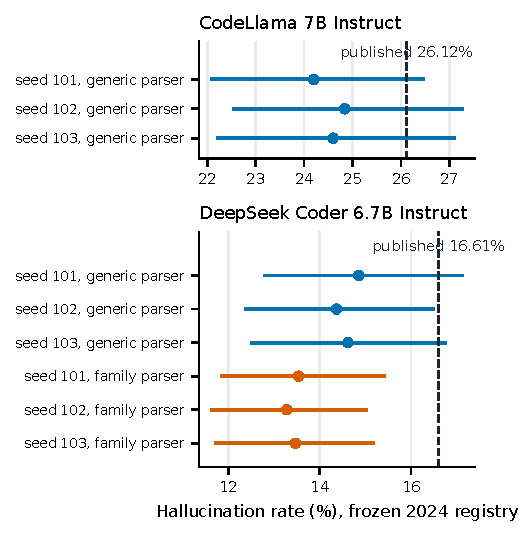
\includegraphics[width=\linewidth]{fig_tracka_forest}
\caption{Track A replication. The dashed line is the published value; each dot is one seed with its
95\% prompt-based confidence interval. The family parser is DeepSeek's original parser, and every
family-parser interval excludes the published value.}
\label{fig:tracka}
\end{figure}

% Generated by paper/build_tables.py -- do not edit by hand.
\begin{table*}[t]
\centering
\scriptsize
\setlength{\tabcolsep}{3pt}
\begin{adjustbox}{max width=\linewidth}
\begin{tabular}{@{}llrrlcrlcrr@{}}
\toprule
Model & Paper (\%) & Seed & Generic (\%) & 95\% CI & $\ni$ paper & Family (\%) & 95\% CI & $\ni$ paper & v2 malformed (\%) & Cap hits \\
\midrule
CodeLlama 7B & 26.12 & 101 & 24.20 & 22.09--26.45 & yes & -- & -- & -- & 10.9 & 54 \\
 &  & 102 & 24.84 & 22.55--27.26 & yes & -- & -- & -- & 8.5 & 60 \\
 &  & 103 & 24.60 & 22.23--27.09 & yes & -- & -- & -- & 13.2 & 64 \\
\quad seed mean &  &  & 24.55 &  &  & -- &  &  &  &  \\
DeepSeek Coder 6.7B & 16.61 & 101 & 14.86 & 12.81--17.12 & yes & 13.54 & 11.86--15.41 & no & 57.6 & 810 \\
 &  & 102 & 14.37 & 12.39--16.49 & no & 13.28 & 11.63--15.01 & no & 58.8 & 813 \\
 &  & 103 & 14.62 & 12.52--16.75 & yes & 13.47 & 11.72--15.17 & no & 58.1 & 816 \\
\quad seed mean &  &  & 14.62 &  &  & 13.43 &  &  &  &  \\
\bottomrule
\end{tabular}
\end{adjustbox}
\par\vspace{2pt}\begin{minipage}{\linewidth}\footnotesize Paper protocol exactly (caps 2048/64, temperature 0.7/0.01, top-$k$ 20, top-$p$ 0.9), one frozen 200-prompt-per-dataset subset, three independent generation seeds per model, frozen 2024-01-10 registry. Intervals are dataset-stratified prompt-cluster bootstraps. The generic parser is the historical parser for CodeLlama; the DeepSeek family parser is the historical parser for DeepSeek and therefore the acceptance condition. Parser~v2 malformed shares are diagnostic; the 64-token cap truncates DeepSeek package queries so often that most of its responses fail the strict grammar. Cap hits are summed over all twelve phases.\end{minipage}
\caption{Track A: seed-level replication estimates against the published values.}
\label{tab:tracka}
\end{table*}


So the ordering and the rough size of the effect reproduce, but the exact DeepSeek value does not.
Both models come out 1.5--2 percentage points low at every seed. That consistent bias points at the
model artifacts themselves: the 2024 study used GPTQ 4-bit weights through \texttt{transformers},
while we used Q4\_0 GGUF weights through Ollama, with possibly different chat templates. We now
record digests so this can be pinned in future, but the 2024 checkpoints cannot be recovered. The
malformed shares in Table~\ref{tab:tracka} also show why the old protocol is hard to reuse. Its
64-token cap on package answers cuts DeepSeek off so often (810--816 cap hits per seed) that most of
its answers fail a strict grammar.

\subsection{Controlled cap diagnostic}
\label{sec:cap}

Our earlier report \citep{anderson2026replication} had found that DeepSeek's measured rate rose by
11.5 percentage points when the token cap was raised, and read that as truncation hiding invented
names at the end of long lists. The independent audit \citep{codex2026audit} found a different
explanation. With more tokens, DeepSeek drifted out of the requested list format (code fences appeared
in 338 of 800 long answers versus 132 of 800 short ones), and the permissive parser then scored code
fragments and prose as invented packages. That finding called for a controlled test. We queried both
DeepSeek models over the same code and prompts at temperature 0 with a fixed seed and one worker,
under caps of 64, 128, 256, 512, and 2048 tokens in counterbalanced order, and checked that shorter
answers were prefixes of longer ones. Parser~v2 scored everything (Figure~\ref{fig:cap}; Appendix
Table~\ref{tab:capcells}).

\begin{figure*}[t]
\centering
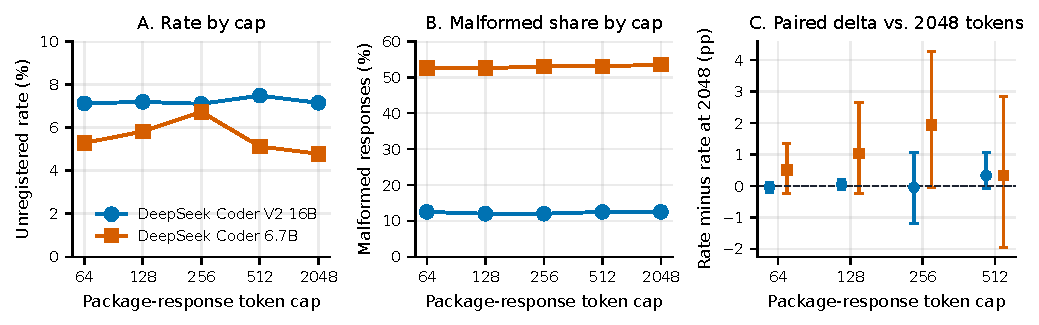
\includegraphics[width=\textwidth]{fig_cap_diagnostic}
\caption{Controlled cap diagnostic. (A) Unregistered rate at each cap on package answers. (B) Share
of malformed answers at each cap. (C) Each cap compared with the 2048-token answer to the same prompt,
with 95\% paired, dataset-stratified bootstrap intervals. Every interval includes zero. No
equivalence margin was preregistered.}
\label{fig:cap}
\end{figure*}

DeepSeek Coder V2 16B scored between 7.10\% and 7.48\% at every cap. No cap differs from the
2048-token cap by more than 0.33 percentage points, and every paired interval includes zero. DeepSeek
Coder 6.7B does not move in one direction either: 5.28\%, 5.81\%, 6.72\%, 5.12\%, and 4.78\%. Every
paired interval includes zero, although the interval at cap 256 is wide ($-0.04$ to $4.29$ percentage
points). The malformed share barely moves with the cap (about 12\% for one model and 53\% for the
other). What the data support is this: the large cap effect from the earlier work does not reappear as
a consistent or monotone effect when decoding is deterministic and the parser is strict. What the
data do not support is a claim of ``no effect.'' We preregistered no equivalence margin, some paired
answers still diverged before the truncation point, and we did not vary temperature along with the
cap. Two earlier findings do still stand: a 64-token cap silently produces empty answers from a
reasoning model (gpt-oss 20B returned nothing on 15 of 15 probe queries, versus 0 of 15 for a
CodeLlama control), and a list cut off at a cap interacts with any parser.

\subsection{Modern benchmark}
\label{sec:trackb}

Table~\ref{tab:trackb} and Figure~\ref{fig:trackb} give the six Track B cells. Three models are low:
Claude Opus 5 at 1.31\% (95\% interval 1.04--1.62), GPT-5.2 at 1.88\% (1.49--2.30), and gpt-oss 20B at
2.15\% (1.76--2.57). DeepSeek Coder V2 16B is high at 10.30\% (8.77--11.89), with the most malformed
answers (18.25\%) and the fewest packages per prompt. Grok 4.6 at 8.22\% and DeepSeek V4 Flash at
17.91\% have intervals so wide (1.55--18.27 and 5.71--29.86) that the point estimates say little on
their own. We do not call Opus, GPT-5.2, and gpt-oss a ``frontier trio.'' gpt-oss is a local 20B
open-weight model, and six hand-picked cells are not a representative sample of anything.

% Generated by paper/build_tables.py -- do not edit by hand.
\begin{table*}[t]
\centering
\scriptsize
\setlength{\tabcolsep}{3pt}
\begin{adjustbox}{max width=\linewidth}
\begin{tabular}{@{}lrlrrrrrrrr@{}}
\toprule
Model & Rate (\%) & 95\% CI & Risk (\%) & Malf.\ (\%) & Empty (\%) & Pkgs/prompt & Parsed & Unique & Top-3 (\%) & Leave-3 (\%) \\
\midrule
Claude Opus 5 & 1.31 & 1.04--1.62 & 12.1 & 3.75 & 0.31 & 11.60 & 9,280 & 95 & 10.7 & 1.18 \\
GPT-5.2 & 1.88 & 1.49--2.30 & 12.1 & 0.56 & 0.00 & 9.03 & 7,222 & 102 & 8.1 & 1.74 \\
gpt-oss 20B & 2.15 & 1.75--2.58 & 13.1 & 0.44 & 6.94 & 7.78 & 6,223 & 91 & 5.2 & 2.05 \\
Grok 4.6 & 8.22 & 1.55--18.27 & 5.5 & 12.56 & 0.06 & 8.44 & 6,754 & 532 & 82.9 & 1.61 \\
DeepSeek Coder V2 16B & 10.30 & 8.77--11.89 & 21.0 & 18.25 & 0.00 & 3.05 & 2,437 & 196 & 4.0 & 9.93 \\
DeepSeek V4 Flash & 17.91 & 5.71--29.86 & 18.1 & 10.38 & 1.00 & 7.57 & 6,054 & 1,045 & 72.4 & 5.71 \\
\bottomrule
\end{tabular}
\end{adjustbox}
\par\vspace{2pt}\begin{minipage}{\linewidth}\footnotesize Rate = unregistered-PyPI recommendation occurrences / Parser~v2-accepted package occurrences (absent from both the 2024-01-10 and 2026-08-12 snapshots and not a standard-library module). Intervals: 50,000-replicate dataset-stratified prompt-cluster percentile bootstrap. Prompt risk = share of the 800 prompts with at least one unregistered recommendation. Top-3 share = share of unregistered occurrences supplied by the three worst responses; leave-3 = rate after removing them (a concentration diagnostic, not an alternative estimand). $n = 1{,}600$ package responses per cell.\end{minipage}
\caption{Track B primary outcomes with response coverage and concentration.}
\label{tab:trackb}
\end{table*}


\begin{figure*}[t]
\centering
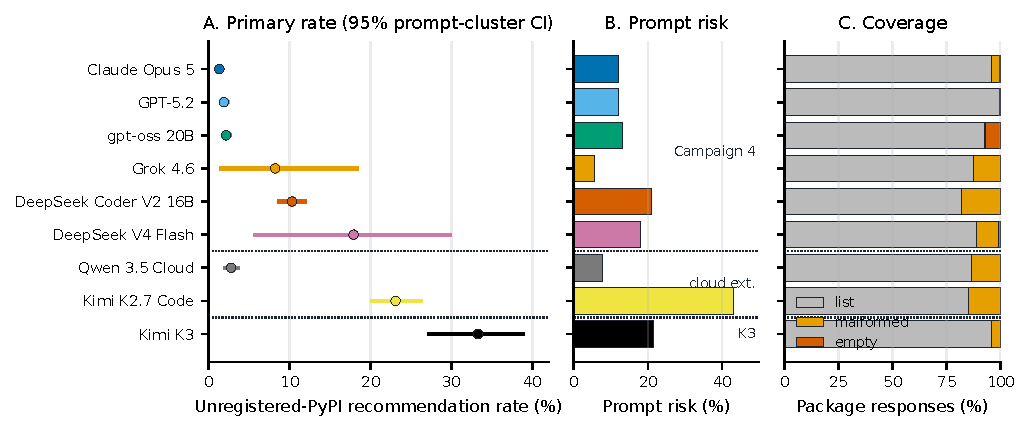
\includegraphics[width=\textwidth]{fig_trackb_forest}
\caption{Rates and response coverage for the six Campaign~4 cells, the two preregistered cloud
extension cells, and the Kimi K3 successor cell. (A) Primary rate with its 95\% prompt-based
interval. (B) Prompt risk. (C) Share of answers that were lists, malformed, or empty. Dotted lines
separate the three families, which were compared under separate Holm corrections.}
\label{fig:trackb}
\end{figure*}

Coverage differs a lot between models. gpt-oss returned 111 empty answers (6.94\%) even with a
2048-token cap. Grok and DeepSeek V4 Flash gave malformed answers 10--13\% of the time, and DeepSeek
Coder V2 18\% of the time. Because malformed answers add nothing to the rate, we never publish a rate
without these columns.

\subsection{Failure regimes and tail risk}
\label{sec:tail}

The central finding is that similar averages can hide very different risks
(Figures~\ref{fig:concentration} and \ref{fig:leavetopk}). If we rank prompts by how many
unregistered names they produced and add up their share, three patterns appear.

\begin{figure*}[t]
\centering
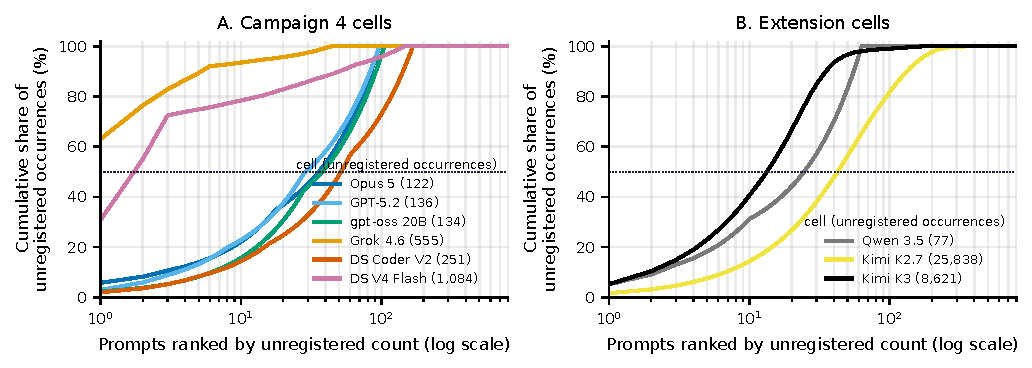
\includegraphics[width=\textwidth]{fig_concentration}
\caption{Concentration curves. Each curve shows what share of a cell's unregistered names comes from
its $k$ worst prompts. (A) Campaign~4 cells. (B) Extension cells. Grok 4.6 and DeepSeek V4 Flash reach
half of their total within one and two prompts; the low-rate cells and DeepSeek Coder V2 need 29--52
prompts.}
\label{fig:concentration}
\end{figure*}

\begin{figure}[t]
\centering
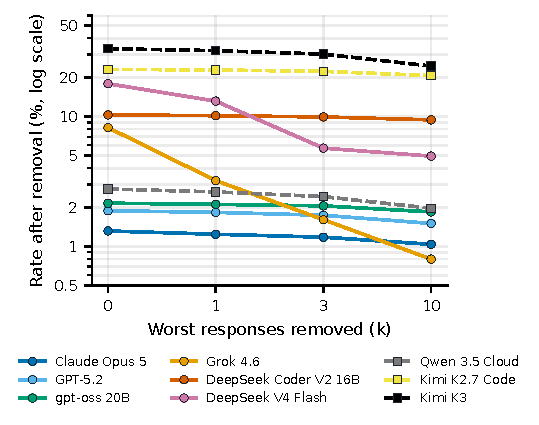
\includegraphics[width=\linewidth]{fig_leave_topk}
\caption{Leave-top-$k$: the rate after removing the $k$ worst answers, for $k$ of 0, 1, 3, and 10.
Flat lines mean the errors are spread out; steep lines mean a few answers dominate. This is a
description of concentration, not a replacement for the primary rate.}
\label{fig:leavetopk}
\end{figure}

\paragraph{Low rate, spread out.} For Opus, GPT-5.2, and gpt-oss, the three worst answers supply
only 5--11\% of unregistered names. Removing them moves the rate by 0.10--0.13 percentage points (1.31
to 1.18, 1.88 to 1.74, 2.15 to 2.05). It takes 29--38 prompts to reach half of each cell's total. The
median prompt has no unregistered name, and the worst prompt has 3--7.

\paragraph{High rate, spread out.} DeepSeek Coder V2's three worst answers supply only 3.98\% of its
unregistered names. Removing them leaves 9.93\%; removing ten leaves 9.43\%. Its problem is
everywhere: 21.0\% of prompts produce at least one unregistered name, the highest prompt risk in the
group.

\paragraph{Catastrophic tail.} A single Grok 4.6 answer, with 350 names in it, supplies 63.06\% of
Grok's unregistered names, and three answers supply 82.88\%. Remove those three and Grok drops from
8.22\% to 1.61\%; remove ten and it is 0.80\%. For DeepSeek V4 Flash, two prompts supply half of the
total, three answers supply 72.42\%, and the rate without them is 5.71\%. Both models have the
\emph{lowest} prompt risk in the group (5.5\% and 18.1\%). A typical Grok or V4 Flash answer is fine;
the tail is a runaway inventory of names. That same concentration is what makes their intervals so
wide.

The practical point is that the same average calls for different defenses. Spread-out errors call for
checking every recommended name against the registry at install time. Catastrophic tails call for
detecting floods, capping the length of recommendation lists, and refusing to enumerate. A leaderboard
that puts Grok 4.6 (8.22\%) next to DeepSeek Coder V2 (10.30\%) hides that they fail in different
ways.

\subsection{Pairwise sensitivity}
\label{sec:pairwise}

Table~\ref{tab:paired} lists all 15 paired comparisons. Seven pass under the preregistered rule, and
five pass under the recentered-null check. Five differences hold up under both:
\begin{itemize}
\item Opus versus gpt-oss ($-0.84$ percentage points, 95\% interval $-1.28$ to $-0.39$);
\item Opus, GPT-5.2, and gpt-oss, each versus DeepSeek Coder V2 (about $-8$ to $-9$ percentage
  points);
\item Opus versus DeepSeek V4 Flash ($-16.59$ percentage points, $-28.65$ to $-4.43$).
\end{itemize}
GPT-5.2 and gpt-oss versus DeepSeek V4 Flash pass the preregistered rule but not the recentered check
(adjusted $p = 0.0596$). Opus versus GPT-5.2 is inconclusive ($-0.57$ percentage points; raw
$p \approx 0.008$, adjusted $\approx 0.07$). An earlier draft had called that pair significant, based
on a bootstrap with 2,000 replicates that did not stratify by dataset; the reviewer's challenge was
verified and adopted. No comparison involving Grok 4.6 survives correction, because a handful of
prompts drive its estimate. We therefore do not rank the six models from best to worst, and we lead
with effect sizes, intervals, and the shape of the tail.

% Generated by paper/build_tables.py -- do not edit by hand.
\begin{table*}[t]
\centering
\footnotesize
\setlength{\tabcolsep}{3pt}
\begin{adjustbox}{max width=\linewidth}
\begin{tabular}{@{}lrlrcrc@{}}
\toprule
Pair & $\Delta$ (pp) & 95\% CI & Holm $p$ (tail) & sig. & Holm $p$ (recent.) & sig. \\
\midrule
Opus 5 vs.\ DS Coder V2 & -8.98 & -10.58---7.45 & 0.0003 & yes & 0.0003 & yes \\
Opus 5 vs.\ DS V4 Flash & -16.59 & -28.65---4.43 & 0.0003 & yes & 0.0453 & yes \\
GPT-5.2 vs.\ DS Coder V2 & -8.42 & -9.98---6.89 & 0.0003 & yes & 0.0003 & yes \\
GPT-5.2 vs.\ DS V4 Flash & -16.02 & -28.17---3.80 & 0.0003 & yes & 0.0596 & no \\
gpt-oss vs.\ DS Coder V2 & -8.15 & -9.71---6.65 & 0.0003 & yes & 0.0003 & yes \\
gpt-oss vs.\ DS V4 Flash & -15.75 & -27.79---3.54 & 0.0003 & yes & 0.0596 & no \\
Opus 5 vs.\ gpt-oss & -0.84 & -1.28---0.39 & 0.0029 & yes & 0.0026 & yes \\
Opus 5 vs.\ GPT-5.2 & -0.57 & -1.00---0.15 & 0.0653 & no & 0.0782 & no \\
Opus 5 vs.\ Grok 4.6 & -6.90 & -16.84---0.24 & 0.1652 & no & 0.5776 & no \\
GPT-5.2 vs.\ Grok 4.6 & -6.33 & -16.39--0.30 & 0.5882 & no & 0.7363 & no \\
gpt-oss vs.\ Grok 4.6 & -6.06 & -16.07--0.56 & 0.7592 & no & 0.7500 & no \\
GPT-5.2 vs.\ gpt-oss & -0.27 & -0.72--0.19 & 0.8656 & no & 0.8402 & no \\
Grok 4.6 vs.\ DS Coder V2 & -2.08 & -9.07--8.02 & 0.8656 & no & 0.8402 & no \\
Grok 4.6 vs.\ DS V4 Flash & -9.69 & -24.43--5.72 & 0.8656 & no & 0.8402 & no \\
DS Coder V2 vs.\ DS V4 Flash & -7.61 & -19.41--4.34 & 0.8656 & no & 0.8402 & no \\
\bottomrule
\end{tabular}
\end{adjustbox}
\par\vspace{2pt}\begin{minipage}{\linewidth}\footnotesize Difference = first minus second model in percentage points on the 800 shared prompts; 50,000-replicate dataset-stratified paired prompt-cluster bootstrap. The bootstrap-tail convention is the preregistered one; the recentered-null convention is a labeled post-hoc sensitivity. Holm correction spans all 15 pairs. Values of 0.0003 sit at the $15 \times 1/50{,}000$ resolution floor and are upper bounds.\end{minipage}
\caption{Track B paired comparisons under both bootstrap conventions.}
\label{tab:paired}
\end{table*}


\subsection{Concurrent-work bridge}
\label{sec:bridge}

Table~\ref{tab:bridge} shows what happens when our outputs are scored the way Churilov scores them.
Under our two-registry, non-stdlib definition, the original six Campaign~4 cells score 8.30\%
(GPT-5.2), 8.87\% (DeepSeek Coder V2), 8.89\% (DeepSeek V4 Flash), 9.52\% (Opus 5), 10.61\% (gpt-oss),
and 17.49\% (Grok 4.6). The extension cells score 6.51\% (Qwen 3.5), 7.38\% (Kimi K2.7), and 8.37\%
(Kimi K3). Only Qwen lands inside Churilov's reported Python range of 5.49--7.27\%; Kimi K2.7 is 0.11
percentage points above its top. The two studies share no model, so we describe this contrast rather
than test it.

% Generated by paper/build_tables.py -- do not edit by hand.
\begin{table*}[t]
\centering
\scriptsize
\setlength{\tabcolsep}{3pt}
\begin{adjustbox}{max width=\linewidth}
\begin{tabular}{@{}lrrrlrlrrr@{}}
\toprule
Model & Mentions & Imports (\%) & Frozen rate (\%) & 95\% CI & Dual rate (\%) & 95\% CI & Cov.\ (\%) & Risk (\%) & Unique \\
\midrule
Claude Opus 5 & 788 & 95.4 & 9.52 & 6.04--13.71 & 9.52 & 6.04--13.71 & 50.5 & 6.1 & 50 \\
GPT-5.2 & 759 & 89.3 & 8.30 & 5.66--11.41 & 8.30 & 5.66--11.41 & 49.2 & 6.0 & 44 \\
gpt-oss 20B & 782 & 92.3 & 10.74 & 8.34--13.28 & 10.61 & 8.22--13.14 & 52.9 & 8.5 & 51 \\
Grok 4.6 & 766 & 98.2 & 18.15 & 12.45--23.92 & 17.49 & 11.91--23.18 & 48.5 & 7.0 & 95 \\
DeepSeek Coder V2 16B & 778 & 95.0 & 9.13 & 7.02--11.38 & 8.87 & 6.80--11.08 & 56.0 & 7.9 & 48 \\
DeepSeek V4 Flash & 742 & 98.9 & 8.89 & 6.73--11.23 & 8.89 & 6.73--11.23 & 52.0 & 7.4 & 44 \\
Qwen 3.5 Cloud & 169 & 98.8 & 7.10 & 3.57--11.05 & 6.51 & 3.12--10.38 & 14.1 & 1.4 & 7 \\
Kimi K2.7 Code & 745 & 96.8 & 7.38 & 5.50--9.46 & 7.38 & 5.50--9.46 & 53.2 & 6.5 & 36 \\
Kimi K3 & 777 & 97.4 & 8.62 & 6.57--10.84 & 8.37 & 6.33--10.57 & 52.6 & 7.2 & 41 \\
\bottomrule
\end{tabular}
\end{adjustbox}
\par\vspace{2pt}\begin{minipage}{\linewidth}\footnotesize Churilov's public extraction design (a \texttt{pip install} regex plus top-level imports, AST-first with a tree-sitter fallback, stdlib-list 3.11 exclusion, and the artifact's false-positive filter) applied to the frozen generated code of every cell; no responses were regenerated. Mentions are the unit of the rate; intervals cluster by prompt and stratify by dataset (50,000 replicates). Across all nine cells, 632 frozen-absence mentions reduce to 621 under the dual-registry/non-stdlib definition (11 removed), and imports supply 97.9\% of dual-registry flags. Coverage = share of prompts with any extracted reference. Churilov's reported Python range is 5.49--7.27\%.\end{minipage}
\caption{Code-import bridge: frozen Campaign 4 and extension outputs rescored with Churilov's extractor.}
\label{tab:bridge}
\end{table*}


Four facts shape the interpretation. First, using the same extractor does not by itself bring the
studies into agreement: on identical outputs, the original six cells stay above the reported band.
Second, registry drift is not the explanation: the 2026 registry and the standard-library rule remove
only 11 of 632 flagged mentions. Third, imports account for 608 of the 621 remaining flags (97.91\%).
Explicit install commands are rare in generated code, so the open question is whether an import can
be mapped straight to a PyPI package at all. Many real packages import under a different name than
they install under, and an import can refer to a file in the same project. Fourth, the prompt source
matters a great deal. Across the nine cells, the LLM-written datasets score 3.70--26.45\% while the
Stack Overflow datasets score 0.00--7.50\% (Appendix Table~\ref{tab:bridgedatasets}). That agrees in
direction with Churilov's observation that synthetic prompts produce higher rates. One caution: Kimi
K2.7's and K3's package-question rates are a different quantity, dominated by extreme \qtwo\ lists,
and must not be compared with code-import rates at all.

\subsection{Prompt-conditioned overlap}
\label{sec:overlap}

Table~\ref{tab:overlap} and Figure~\ref{fig:overlap} separate ordinary overlap from overlap on the
same prompt. Among the six Campaign~4 cells, five unregistered names are produced by every model, but
four of those five are produced by all six models on at least one identical prompt. Across all nine
cells, the average Jaccard similarity between pairs is 0.038, two names appear in every model, and one
of the two appears in every model on the same prompt. For most pairs, 60--95\% of the names they
share occur on a shared prompt; the share drops only where a Kimi flood is involved (Appendix
Table~\ref{tab:overlappairs}). Ordinary overlap cannot tell whether two models share a name because
they share training data, because a package by that name is a common misconception, or because the
same prompt pulled it out of both. The aligned numbers show that the prompt is a live explanation. It
has to be ruled out before overlap can be read as evidence about training data.

% Generated by paper/build_tables.py -- do not edit by hand.
\begin{table}[t]
\centering
\footnotesize
\setlength{\tabcolsep}{3pt}
\begin{adjustbox}{max width=\linewidth}
\begin{tabular}{@{}p{5.6cm}rr@{}}
\toprule
Overlap statistic & Six cells & Nine cells \\
\midrule
Mean pairwise ordinary name Jaccard & 0.054 & 0.038 \\
Names emitted by every model & 5 & 2 \\
\quad of which emitted by every model on one identical prompt & 4 & 1 \\
\quad same-prompt share of the universal set (\%) & 80 & 50 \\
\bottomrule
\end{tabular}
\end{adjustbox}
\par\vspace{2pt}\begin{minipage}{\linewidth}\footnotesize Base set: dual-registry, non-stdlib unregistered recommendations accepted by Parser~v2. The six-cell column is the frozen Campaign~4 cohort (artifact at commit \texttt{a212e05}, \texttt{eac1434} before the 2026-09-27 history rewrite); the nine-cell column adds the three extension cells. Candidate names are withheld.\end{minipage}
\caption{Ordinary versus prompt-aligned cross-model overlap.}
\label{tab:overlap}
\end{table}


\begin{figure*}[t]
\centering
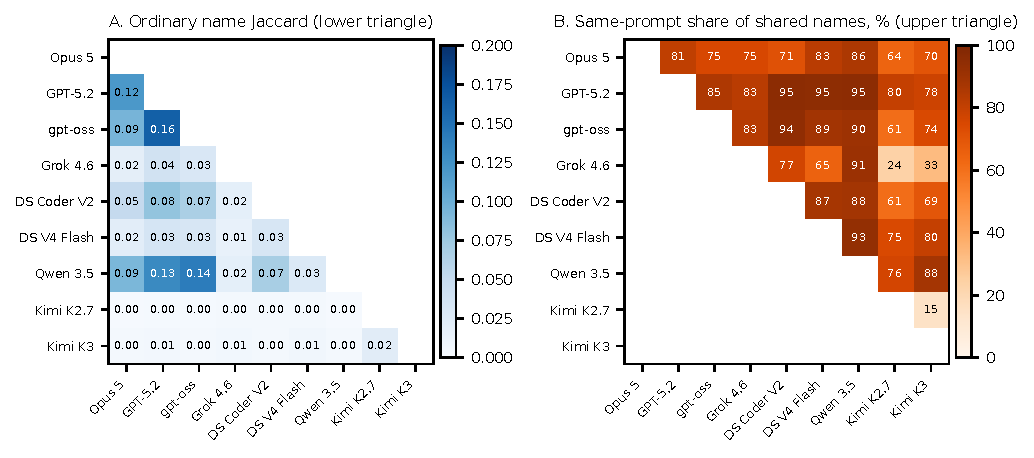
\includegraphics[width=\textwidth]{fig_overlap}
\caption{Ordinary versus prompt-aligned overlap among the nine cells. (A) Jaccard similarity of the
sets of unregistered names. (B) Share of each pair's shared names that both models produced on at
least one identical prompt. Kimi's flood-inflated name sets drive its low ordinary Jaccard.}
\label{fig:overlap}
\end{figure*}

\subsection{Preregistered Qwen/Kimi cloud extension}
\label{sec:extension}

Table~\ref{tab:extension} reports the two preregistered cloud cells, and Appendix
Table~\ref{tab:extpairs} their family of 13 comparisons (10 pass the preregistered rule, 9 the
recentered check). Qwen 3.5 Cloud is clean: 2.77\% (2.07--3.54), 7.88\% prompt risk, 13.25\% malformed
answers, no package answer at the token cap, and 2,782 accepted names. Kimi K2.7 Code Cloud is
23.10\% (20.19--26.19), with 43.00\% prompt risk, 14.75\% malformed answers, 323 package answers at
the cap, and 111,842 accepted names, of which 107,955 come from \qtwo.

% Generated by paper/build_tables.py -- do not edit by hand.
\begin{table}[t]
\centering
\footnotesize
\setlength{\tabcolsep}{3pt}
\begin{adjustbox}{max width=\linewidth}
\begin{tabular}{@{}p{4.3cm}>{\raggedleft\arraybackslash}p{1.6cm}>{\raggedleft\arraybackslash}p{2.1cm}@{}}
\toprule
Outcome & Qwen 3.5 Cloud & Kimi K2.7 Code \\
\midrule
Unregistered recommendation rate (\%) & 2.77 & 23.10 \\
\quad 95\% prompt-cluster interval & 2.07--3.54 & 20.19--26.19 \\
Prompt risk (\%) & 7.88 & 43.00 \\
Malformed / empty responses (\%) & 13.25 / 0.00 & 14.75 / 0.00 \\
Parsed package occurrences & 2,782 & 111,842 \\
Unregistered occurrences & 77 & 25,838 \\
Unique unregistered names & 71 & 21,631 \\
Cap hits: code / package responses & 1 / 0 & 10 / 323 \\
Query 1 rate (\%) / occurrences & 0.33 / 302 & 21.82 / 3,887 \\
Query 2 rate (\%) / occurrences & 3.06 / 2,480 & 23.15 / 107,955 \\
Responses with $\leq 10$ packages: rate (\%) & 2.82 & 4.95 \\
Responses with $> 25$ packages: rate (\%) / occurrences & 0.00 / 31 & 23.93 / 106,980 \\
Response-macro mean / median (\%) & 3.23 / 0.00 & 8.36 / 0.00 \\
Prompt-macro mean / median (\%) & 3.75 / 0.00 & 11.78 / 0.00 \\
Top-3 response share (\%) & 13.0 & 4.6 \\
Cap-proxy-excluded rate (\%) [post hoc] & 2.77 & 13.18 \\
Tokens: prompt / completion & 731,235 / 92,619 & 1,026,611 / 1,134,677 \\
\bottomrule
\end{tabular}
\end{adjustbox}
\par\vspace{2pt}\begin{minipage}{\linewidth}\footnotesize Both cells: the Campaign~4 fixed 800-prompt subset, Parser~v2, dual registries, caps 4096/2048, \texttt{think:false}, 2,400 calls each with zero request errors. The cap proxy is the frozen within-phase longest-response proxy because the first extension runner retained cap counts only at phase level; it is explicitly post hoc.\end{minipage}
\caption{Preregistered Qwen 3.5 / Kimi K2.7 extension outcomes with query volume and cap sensitivity.}
\label{tab:extension}
\end{table}


The two questions have to be looked at separately. Kimi's \qone\ rate is 21.82\% over 3,887 names and
its \qtwo\ rate is 23.15\% over 107,955. Even the \qone\ figure is driven by six answers that run
past position 100; leaving out the longest answers in each phase (our stand-in for cap hits) brings it
to 3.77\%. Answers with at most ten packages score 4.95\%. Answers with more than 25 packages supply
106,980 names at 23.93\%. The weighting matters: the pooled rate is 23.10\%, but the average rate per
answer is 8.36\%, the average per prompt is 11.78\%, and the median of both is zero. These are
descriptions, not replacements for the preregistered estimate.

\begin{figure*}[t]
\centering
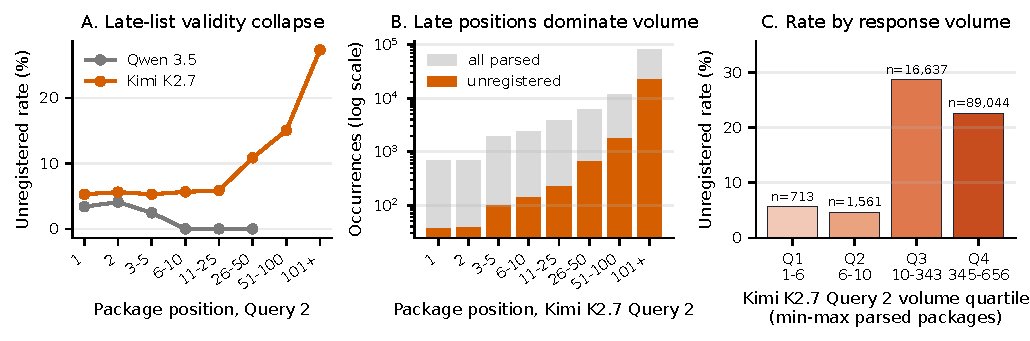
\includegraphics[width=\textwidth]{fig_k27_mechanism}
\caption{Kimi K2.7's rate is a story about long lists. (A) \qtwo\ rate by list position. Kimi stays
near 5--6\% through position 25 and rises to 27.33\% after position 100; Qwen 3.5 produces nothing
after position 50. (B) Most of Kimi's \qtwo\ names sit past position 100 (log scale). (C) The two
longest quartiles of answers carry both the volume and the higher rates. Counts are accepted names,
not prompts.}
\label{fig:k27}
\end{figure*}

List position is the clearest mechanism (Figure~\ref{fig:k27}; Appendix Table~\ref{tab:positions}).
Kimi's \qtwo\ rate is 5.28--5.87\% through position 25, then 10.85\% at positions 26--50, 15.03\% at
51--100, and 27.33\% after 100. This is a model that sometimes ignores the instruction and enumerates,
and whose lists get worse the longer they run; it is not a flat rate. Parser noise plays a part but
does not explain it. The 323 answers we treat as cap hits are malformed 26.94\% of the time, versus
11.67\% for the rest, and they hold 36.86\% of all Kimi's malformed answers. Yet 236 of them do parse
as lists and supply 104,420 names. Even after all 323 are removed, \qtwo\ still climbs from roughly
5--7\% through position 25 to 22.03\%, 36.94\%, and 41.38\% at positions 26--50, 51--100, and 101+.
Those late bins rest on only 16, 12, and 10 answers, so they show the mechanism rather than measure it
precisely. The 234 \qtwo\ answers with more than 100 packages are not copies of one list: their mean
pairwise Jaccard is 0.066, a core of 39 names recurs, and the rest varies with the prompt. The
paired \qone/\qtwo\ Jaccard for these floods is only 0.005. Because K2.7's runner did not record which
answers hit the cap, every statement above that depends on the cap is a post-hoc approximation. The
K3 cell was instrumented to remove that ambiguity.

\subsection{Kimi K3 successor test}
\label{sec:k3}

The Kimi K3 cell of 2,400 calls passed all twelve checks on its per-answer records: one served model
id, no errors or request adjustments, 72 exact cap hits (46 of them in package answers, all in
\qtwo), and \$16.27 of token-based spend (Table~\ref{tab:k3}). Its primary rate is 33.30\%
(27.22--38.81), with 21.50\% prompt risk, 4.19\% malformed answers, and 25,889 accepted names. All
eight comparisons in its family put K3 above the other model on this rate (Appendix
Table~\ref{tab:k3pairs}); K2.7 minus K3 is $-10.20$ percentage points ($-16.43$ to $-3.44$).

% Generated by paper/build_tables.py -- do not edit by hand.
\begin{table}[t]
\centering
\footnotesize
\setlength{\tabcolsep}{3pt}
\begin{adjustbox}{max width=\linewidth}
\begin{tabular}{@{}p{5.3cm}>{\raggedleft\arraybackslash}p{2.8cm}@{}}
\toprule
Outcome & Kimi K3 \\
\midrule
Combined unregistered recommendation rate (\%) & 33.30 \\
\quad 95\% prompt-cluster interval & 27.22--38.81 \\
Prompt risk (\%) & 21.50 \\
List coverage / malformed / empty (\%) & 95.81 / 4.19 / 0.00 \\
Parsed / unregistered occurrences & 25,889 / 8,621 \\
Response-macro mean / prompt-macro mean (\%) & 4.18 / 5.78 \\
Query 1 rate (\%) / occurrences & 1.76 / 1,303 \\
Query 2 rate (\%) / occurrences & 34.97 / 24,586 \\
Responses with $\leq 10$ packages: rate (\%) & 2.67 \\
Responses with $> 25$ packages: rate (\%) / occurrences & 43.62 / 19,227 \\
Exact cap hits: all phases / package responses & 72 / 46 \\
Package cap hits: share of responses / parsed / unregistered (\%) & 2.88 / 51.79 / 81.02 \\
Rate within package cap hits (\%) & 52.10 \\
Rate excluding package cap hits (\%) [post hoc] & 13.11 \\
Top-3 / top-10 response share (\%) & 14.88 / 40.59 \\
\midrule
\multicolumn{2}{@{}l}{\textit{Response-metadata gate}} \\
Ordered sidecar rows / missing & 2,400 / 0 \\
Served model ids & \texttt{kimi-k3} only \\
Request errors / request adjustments & 0 / none \\
Prompt / completion tokens & 1,410,107 / 802,768 \\
Token-derived analytic spend (smoke excluded) & \$16.271841 \\
\bottomrule
\end{tabular}
\end{adjustbox}
\par\vspace{2pt}\begin{minipage}{\linewidth}\footnotesize Design attested as fixed before outcome inspection, but not committed before collection; provenance and completion-gate code changed during collection and before scoring. The prespecified 33.30\% estimate remains primary; cap-hit exclusion is post-hoc conditioning on a post-treatment variable.\end{minipage}
\caption{Kimi K3 successor cell: prespecified outcomes and the exact response-metadata audit.}
\label{tab:k3}
\end{table}


The two questions could not be more different: \qone\ is 1.76\% over 1,303 names and \qtwo\ is
34.97\% over 24,586. K3 answers the question about its own code well, and sometimes treats the
open-ended question as an invitation to list everything. The exact cap records explain the headline.
The 46 package answers that hit the cap are 2.88\% of package answers, but they supply 13,408 names
(51.79\% of all accepted names) and 6,985 unregistered names (81.02\% of the total), at a rate of
52.10\% within those answers. Without them the rate would be 13.11\%. We keep 33.30\% as the primary
result. Whether an answer hit the cap is only known after the answer was generated, so removing those
answers is conditioning on an outcome \citep{montgomery2018conditioning}, and we label it a
diagnostic, not a correction.

% Generated by paper/build_tables.py -- do not edit by hand.
\begin{table}[t]
\centering
\scriptsize
\setlength{\tabcolsep}{3pt}
\begin{adjustbox}{max width=\linewidth}
\begin{tabular}{@{}p{4.0cm}>{\raggedleft\arraybackslash}p{2.2cm}>{\raggedleft\arraybackslash}p{2.0cm}@{}}
\toprule
Diagnostic & Kimi K2.7 & Kimi K3 \\
\midrule
\multicolumn{3}{@{}l}{\textit{Aggregate decomposition (all package responses)}} \\
Occurrence-weighted rate (\%) & 23.10 & 33.30 \\
Prompt risk (\%) & 43.00 & 21.50 \\
Response-macro mean (\%) & 8.36 & 4.18 \\
Responses with $\geq 100$ packages & 240 & 54 \\
Package cap hits (K2.7: proxy; K3: exact) & 323 & 46 \\
\quad share of responses / parsed / unregistered (\%) & 20.2 / 93.4 / 96.2 & 2.9 / 51.8 / 81.0 \\
Rate inside the cap tail (\%) & 23.81 & 52.10 \\
Rate excluding the cap tail (\%) [post hoc] & 13.18 & 13.11 \\
\midrule
\multicolumn{3}{@{}l}{\textit{Shared-prompt Query 2 diagnostics (K2.7 minus K3, pp; 95\% paired CI)}} \\
Prompt risk & 41.12\% vs.\ 20.50\% & 20.62 (16.50--24.75) \\
Responses over 100 packages & 29.25\% vs.\ 6.75\% & 22.50 (19.00--26.00) \\
Flood contingency (both / K2.7 only / K3 only / neither) & 22 / 212 / 32 / 534 &  \\
Expected joint floods under independence; odds ratio & 15.8; 1.73 &  \\
Flood-prompt Jaccard; maximum given marginals & 0.083; 0.231 &  \\
\midrule
\multicolumn{3}{@{}l}{\textit{K3 flood diversity (54 Query 2 responses above 100 packages)}} \\
Unique normalized packages / unregistered names & 12,127 / 8,010 &  \\
Mean pairwise Jaccard: package sets / unregistered sets & 0.0408 / 0.0011 &  \\
Unregistered names in $\geq 25\%$ of floods & 0 &  \\
\bottomrule
\end{tabular}
\end{adjustbox}
\par\vspace{2pt}\begin{minipage}{\linewidth}\footnotesize K3 cap membership is exact (finish reason and token counts per response); K2.7 cap membership is the frozen within-phase longest-response proxy. Paired intervals resample prompts within each of the four 200-prompt datasets (50,000 replicates). Cap exclusion is diagnostic conditioning, not a causal estimate.\end{minipage}
\caption{Kimi K2.7 versus Kimi K3: aggregation decomposition, shared-prompt flood contingency, and cap-tail influence.}
\label{tab:k27k3}
\end{table}


Compared with K2.7, the ranking flips depending on the metric (Table~\ref{tab:k27k3},
Figure~\ref{fig:k3}). K3 has lower prompt risk (21.50\% versus 43.00\%), a lower average rate per
answer (4.18\% versus 8.36\%), and only 54 \qtwo\ answers above 100 packages versus 234. On the 800
shared prompts, the paired difference in \qtwo\ prompt risk is 20.63 percentage points
(16.50--24.75), and the difference in flood frequency is 22.50 percentage points (19.00--26.00). Yet
K3's rarer floods are much worse (52.10\% unregistered, versus 23.81\% in K2.7's approximate cap
hits), so its pooled rate is higher. Set aside the cap tails of both, as a diagnostic, and the two
rates nearly coincide: 13.11\% and 13.18\%. Twenty-two prompts flood in both models, against 15.8
expected if flooding were independent (odds ratio 1.73), so some prompts are prone to floods in both.
But the Jaccard overlap of flood prompts is 0.083 against a maximum of 0.231 given the two models'
flood rates, so the prompt alone does not decide which model floods. The 54 K3 floods contain 8,010
distinct unregistered names with a mean pairwise Jaccard of 0.0011, and no name appears in even a
quarter of them. The tail is not one memorized list repeated, and it is not a parser stuck in a loop.
That does not remove the parser's ordinary limitations.

\begin{figure*}[t]
\centering
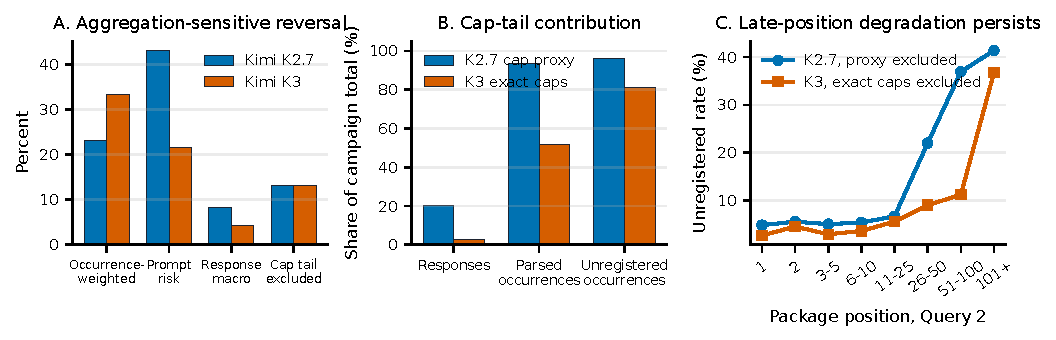
\includegraphics[width=\textwidth]{fig_k3_mechanism}
\caption{Kimi K2.7 versus Kimi K3. (A) The ranking depends on the metric: K3 is worse when every name
counts equally, but better on prompt risk, on the average rate per answer, and after cap-tail
exclusion. (B) K3's 46 exact package cap hits are 2.9\% of its answers but 81.0\% of its unregistered
names. (C) Rates still rise with list position after removing the K2.7 approximate cap hits and the
exact K3 cap hits.}
\label{fig:k3}
\end{figure*}

The rise with list position survives the removal of exact cap hits: K3's \qtwo\ rate goes from
2.70--5.62\% through position 25 to 9.06\%, 11.22\%, and 36.75\% at positions 26--50, 51--100, and
101+. So the mechanism has two stages. Occasionally the model runs away and enumerates, and the
further down the list it gets, the less real the names become. The token cap reveals that process and
cuts it off; nothing here shows that the cap causes it.

\section{Discussion}
\label{sec:discussion}

\subsection{The parser is part of the measurement instrument}

Strict parsing bought precision by refusing unclear answers, and the cost was visible: 79.75\% recall
in validation, and malformed shares from 0.44\% (gpt-oss) to 18.25\% (DeepSeek Coder V2) in the
benchmark. Differences that large can bias a comparison between models if they are left out, because
the rate of a low-coverage model is computed only from the answers that stayed in format. Control
tokens leaked by the transport layer should be stripped before parsing and logged. The Grok
\texttt{<|eos|>} case shows that a hosted endpoint can move a malformed rate by eleven points without
moving the primary rate at all.

\subsection{Registry time changes the label space}

A name can move from ``hallucinated'' to registered, or from registered to deleted, with no change in
the model, and the 2024 registry contained squatted standard-library names that hid module confusion
entirely. Registry snapshots should be dated and hashed like model weights, and rates should be scored
against both a frozen and a current snapshot with an explicit standard-library rule. The bridge adds a
corollary: with the extractor held fixed, registry drift explains almost none of the gap between the
two studies, so a disagreement between two 2026 rates is about which models, which prompts, and how
names are extracted, not about the calendar.

\subsection{Average rates conceal operationally different risks}

Six modern models showed three kinds of failure: low and spread out, high and spread out, and
catastrophic tail. Security evaluations need tail-aware metrics because the defenses differ.
Spread-out risk is handled by checking names against the registry at install time and by asking the
user to confirm installations. Catastrophic tails are handled by flood guards and by bounding how
many names a model may recommend. The K2.7/K3 comparison is the clearest example: K3 is the safer
model on a typical prompt and the worse model when every emitted name counts equally. Neither number
contains the other. A report that carries only one of them answers only one operational question.

\subsection{What the cap diagnostic resolves, and what it does not}

Under deterministic decoding and a strict parser, the proposed cap mechanism for DeepSeek is weakened:
rates are flat or non-monotone across a 32-fold range of caps, and every paired interval includes
zero. The diagnostic does not show that temperature caused the earlier association
\citep{anderson2026replication}, and it does not prove equivalence. The exact K3 cap records then
show a different relationship between caps and outcomes: answers that hit the cap can dominate a rate,
but cap status is only known after generation, so it cannot separate a runaway list from the boundary
that truncates it. A randomized within-prompt cap experiment is still needed.

\subsection{Replication as measurement debugging}

The useful verdict is not a yes or a no. Whether the transport reproduces the artifact, whether the
instrument measures package recommendations, and what current models do are three separate
questions with separate evidence. ``The pattern reproduces but the exact number does not'' is more
informative than ``replicated'' or ``failed to replicate,'' because it places the leftover gap in the
model artifacts rather than in the phenomenon. And that gap only became visible once the parser and
cap confounds were removed.

\subsection{What the concurrent replication changes}

Churilov establishes breadth and a real, registrable cross-model attack surface. Our bridge shows that
using the same extractor is necessary but not sufficient for two rates to be comparable. The models,
the prompt source, the mapping from import to package, the refusal policy, and the unit of inference
all still matter. Prompt-conditioned overlap should become standard before a set of universal names
is read as evidence of shared training data, because four of the five all-model names in our cohort
are explained by a shared prompt. Two additions would strengthen that study without any new model
runs: the current-registry check it defers to future work, and a recomputation of its pairwise tests
that clusters by generation.

\section{Threats to validity and limitations}
\label{sec:threats}

\begin{itemize}
\item Python only, and a package-question task rather than general code generation.
\item The six benchmark cells, the two extension cells, and the K3 cell were chosen by hand. They are
  not a representative sample of frontier or local models.
\item Kimi K3's scientific design was frozen, but the provenance and completeness checks were
  expanded during collection; the finished manifest lacks fields added later, which confirms that the
  running process used the earlier code. Those edits did not touch prompts, responses, parsing, or
  outcomes, but ``frozen pipeline'' would overstate the record. The K3 freeze rests on an attestation
  and a later commit, not on a tamper-evident commit made before the data existed.
\item One fixed prompt subset and one generation per model in Track B; only Track A's seeds tell us
  how much a rerun would move.
\item Parser~v2 found 79.75\% of visible recommendations in the validation sample. The Track B audit
  was done by an AI reviewer at the maintainer's direction; no human read every record.
\item The occurrence rate is computed only over names the parser accepted.
\item Hosted aliases and provider infrastructure can change even when the served id is recorded. The
  DeepSeek Coder V2 run was resumed under mixed settings.
\item Some package answers hit the token cap, so the catastrophic-tail totals may be lower bounds.
\item Kimi K2.7's cap counts exist only per phase, so its cap analysis uses the longest answers as a
  stand-in. K3's cap status is exact, but removing cap hits is still conditioning on an outcome, and
  the K2.7/K3 comparison mixes exact labels with a stand-in.
\item Kimi K2.7's rate is dominated by extreme \qtwo\ lists. The occurrence rate and prompt risk
  answer different questions.
\item Unregistered PyPI names include real packages from other ecosystems, not only invented strings.
\item Every tail, control-token, sentinel, recentered-bootstrap, bridge, and cap-conditioning analysis
  was done after seeing the data and is labeled that way. The bridge cohorts share no model, and
  generated imports can refer to local files.
\item The Qwen 3.5 and Kimi K2.7 cells were preregistered separately and are not folded back into
  Campaign~4's original set of comparisons.
\end{itemize}

We also list claims that the evidence does not support:
\begin{itemize}
\item That frontier models hallucinate at 1.3--2.2\%. Grok 4.6 and DeepSeek V4 Flash contradict it,
  and gpt-oss is not a hosted frontier model.
\item That the cap effect ``vanished.'' The diagnostic shows non-reproduction, not the absence of any
  effect.
\item That every unregistered name is invented.
\item That more than five model pairs are definitively different.
\item That Parser~v2 is semantically perfect. Its grammar is reliable, but strict abstention, leaked
  control tokens, and collapsed ``no packages'' tokens are measurable limitations.
\item That Churilov's results and ours agree once extraction is matched.
\item That universal names prove shared training data.
\item That Kimi K2.7 has an ordinary recommendation rate of 23.10\%, or that removing cap hits
  ``repairs'' it.
\item That Kimi K3 is simply worse than K2.7. The ranking depends on the question.
\item That the token cap causes K3's tail.
\item That the low overlap of flood prompts makes prompt susceptibility irrelevant.
\end{itemize}

\section{Security, ethics, and responsible artifact release}
\label{sec:ethics}

Publishing a list of unregistered candidate names would hand attackers a target list. Following the
original study, this paper and every committed artifact release counts, hashes, manifests, model ids
and digests, the parser version, and the registry snapshot identities, but never the names. Raw
responses are kept outside version control under a content-addressed index and can be shared with
verified researchers under a responsible-access policy. This work measures unsafe recommendations. It
does not show that any named package is malicious, and a name registered after a model first
recommended it cannot be distinguished here from an unrelated coincidence.

\section{Conclusion}
\label{sec:conclusion}

The 2024 pattern comes back, but the exact DeepSeek value does not under its own parser. Modern
models fail in distinct ways, spread out or in catastrophic tails, and a single average hides the
difference; a successor model can be safer on typical prompts while scoring worse overall. Future
evaluations of package hallucination should record the registry and parser versions, report how
many answers the parser accepted, build confidence intervals on prompts, and measure how concentrated
the errors are. The next experiment these results call for is a within-prompt factorial that varies
the token cap and adds a bounded-list instruction, launched through the commit-based freeze gate, to
separate runaway enumeration from truncation and to test a practical defense.

\section*{Disclosure of AI involvement}

The code, analyses, and reports in the underlying repository were produced by Anthropic Claude
(Opus 5 and Fable 5) and OpenAI Codex under the interactive direction of the author. The two AI
systems also performed the delegated label sign-off, the Track B parser audit, and two adversarial
reviews of each other's work, and every adopted finding was re-verified against raw artifacts as
committed code. This manuscript was written by Claude (Fable 5.1) from the committed artifacts and
the maintainer's paper outline, and all tables are generated programmatically from the frozen result
files. The maintainer's preregistration sign-offs and delegations are the human control points. The
original study, its pipeline, prompt corpus, and detection code are the work of Spracklen et al.

\bibliographystyle{plainnat}
\bibliography{refs}

% The appendix is typeset in one column so that its wide tables sit where they are introduced.
\clearpage
\onecolumn
\appendix

\section{Artifact checklist}
\label{app:artifacts}

The repository accompanying this paper contains:
\begin{itemize}
\item the full preregistrations and their dated amendments
  (\texttt{Experiments/PREREGISTRATION\_v4.md}, \texttt{PREREGISTRATION\_OLLAMA\_CLOUD\_EXTENSION.md},
  \texttt{PREREGISTRATION\_KIMI\_K3\_EXTENSION.md});
\item the frozen Parser~v2 grammar and its unit tests (\texttt{parser\_v2.py});
\item the initial and Track B audit designs, signed summaries, and hashes;
\item the construction, dates, and counts of both registry snapshots;
\item all seed-level Track A tables and the full cap pairing and position-band tables
  (\texttt{campaign4\_results.json}, \texttt{cap\_diagnostic\_summary.json});
\item all 15 paired comparisons under both conventions (\texttt{campaign4\_post\_analysis.json});
\item prompt-level derived counts sufficient to reproduce every interval without exposing raw names;
\item the DeepSeek Coder V2 run-history addendum;
\item the Churilov-compatible extractor port and its machine-readable output
  (\texttt{churilov\_bridge\_analysis.py}, \texttt{.json});
\item the separately frozen extension protocol, manifests, and post-analysis
  (\texttt{ollama\_cloud\_extension\_results.json}, \texttt{ollama\_cloud\_extension\_post\_analysis.json});
\item the Kimi K3 per-answer metadata records, cost ledger, scoring gate, and results
  (\texttt{kimi\_k3\_extension\_results.json});
\item the K2.7/K3 paired post-analysis (\texttt{kimi\_k2\_7\_vs\_k3\_post\_analysis.json});
\item the retrospective provenance stamp, with its explicit statement that it is not a
  cryptographic preregistration, and the raw-artifact hash index;
\item the review amendment ledger; and
\item the commit-based freeze gate (\texttt{experiment\_gate.py}) required for every future analytic
  run.
\end{itemize}
The manuscript's tables and figures are regenerated from these files by
\texttt{paper/build\_tables.py} and \texttt{paper/make\_figures.py}.

\section{Additional cap-diagnostic tables}
\label{app:cap}

Table~\ref{tab:capcells} lists every paired cell of the controlled cap diagnostic, and
Table~\ref{tab:capbands} the rates by list position within answers that parsed as lists.

% Generated by paper/build_tables.py -- do not edit by hand.
\begin{table}[H]
\centering
\footnotesize
\setlength{\tabcolsep}{3pt}
\begin{adjustbox}{max width=\linewidth}
\begin{tabular}{@{}llrrrrrl@{}}
\toprule
Model & Cap & Packages & Unreg. & Rate (\%) & Malformed (\%) & $\Delta$ vs.\ 2048 (pp) & 95\% CI \\
\midrule
DeepSeek Coder V2 16B & 64 & 323 & 23 & 7.12 & 12.5 & -0.02 & -0.20--0.11 \\
 & 128 & 320 & 23 & 7.19 & 12.0 & 0.04 & -0.11--0.21 \\
 & 256 & 324 & 23 & 7.10 & 12.0 & -0.04 & -1.19--1.06 \\
 & 512 & 321 & 24 & 7.48 & 12.5 & 0.33 & -0.08--1.05 \\
 & 2048 & 322 & 23 & 7.14 & 12.5 & ref. &  \\
\quad Spearman $\rho$ (rate vs.\ cap) &  &  &  & 0.30 &  &  &  \\
DeepSeek Coder 6.7B & 64 & 265 & 14 & 5.28 & 52.5 & 0.50 & -0.23--1.35 \\
 & 128 & 258 & 15 & 5.81 & 52.5 & 1.03 & -0.25--2.66 \\
 & 256 & 238 & 16 & 6.72 & 53.0 & 1.94 & -0.04--4.29 \\
 & 512 & 254 & 13 & 5.12 & 53.0 & 0.34 & -1.94--2.83 \\
 & 2048 & 251 & 12 & 4.78 & 53.5 & ref. &  \\
\quad Spearman $\rho$ (rate vs.\ cap) &  &  &  & -0.60 &  &  &  \\
\bottomrule
\end{tabular}
\end{adjustbox}
\par\vspace{2pt}\begin{minipage}{\linewidth}\footnotesize 100 prompts (25 per dataset), both package queries, temperature 0, seed 7, one worker, counterbalanced cap order, Parser~v2, frozen 2024 registry. Deltas pair each cap with the 2048-token response at the prompt level (20,000-replicate dataset-stratified bootstrap). No equivalence margin was preregistered, so a small delta is not proof of no effect.\end{minipage}
\caption{Controlled cap diagnostic: paired cells.}
\label{tab:capcells}
\end{table}

% Generated by paper/build_tables.py -- do not edit by hand.
\begin{table}[H]
\centering
\scriptsize
\setlength{\tabcolsep}{3pt}
\begin{adjustbox}{max width=\linewidth}
\begin{tabular}{@{}lllrrrrr@{}}
\toprule
Model & Cap & Query & Pos.\ 1 & Pos.\ 2 & Pos.\ 3 & Pos.\ 4 & Pos.\ 5+ \\
\midrule
DeepSeek Coder V2 16B & 64 & Q1 & 6.5\% (n=92) & 3.6\% (n=55) & 10.0\% (n=10) & 33.3\% (n=3) & 0.0\% (n=1) \\
 & 64 & Q2 & 7.3\% (n=82) & 9.1\% (n=66) & 10.0\% (n=10) & 0.0\% (n=4) & -- \\
 & 128 & Q1 & 6.5\% (n=92) & 3.7\% (n=54) & 10.0\% (n=10) & 33.3\% (n=3) & 0.0\% (n=1) \\
 & 128 & Q2 & 7.2\% (n=83) & 9.1\% (n=66) & 12.5\% (n=8) & 0.0\% (n=3) & -- \\
 & 256 & Q1 & 6.5\% (n=92) & 3.6\% (n=55) & 10.0\% (n=10) & 33.3\% (n=3) & 0.0\% (n=1) \\
 & 256 & Q2 & 7.2\% (n=83) & 9.1\% (n=66) & 0.0\% (n=9) & 0.0\% (n=4) & 100.0\% (n=1) \\
 & 512 & Q1 & 7.6\% (n=92) & 3.6\% (n=55) & 10.0\% (n=10) & 33.3\% (n=3) & 0.0\% (n=1) \\
 & 512 & Q2 & 7.3\% (n=82) & 9.2\% (n=65) & 11.1\% (n=9) & 0.0\% (n=4) & -- \\
 & 2048 & Q1 & 6.5\% (n=92) & 3.7\% (n=54) & 10.0\% (n=10) & 33.3\% (n=3) & 0.0\% (n=1) \\
 & 2048 & Q2 & 7.2\% (n=83) & 9.1\% (n=66) & 11.1\% (n=9) & 0.0\% (n=4) & -- \\
DeepSeek Coder 6.7B & 64 & Q1 & 6.2\% (n=64) & 0.0\% (n=39) & 18.8\% (n=16) & 12.5\% (n=8) & 16.7\% (n=6) \\
 & 64 & Q2 & 6.7\% (n=30) & 0.0\% (n=26) & 6.2\% (n=16) & 9.1\% (n=11) & 2.0\% (n=49) \\
 & 128 & Q1 & 7.8\% (n=64) & 0.0\% (n=39) & 18.8\% (n=16) & 12.5\% (n=8) & 16.7\% (n=6) \\
 & 128 & Q2 & 6.9\% (n=29) & 0.0\% (n=25) & 0.0\% (n=15) & 10.0\% (n=10) & 4.3\% (n=46) \\
 & 256 & Q1 & 7.9\% (n=63) & 0.0\% (n=38) & 20.0\% (n=15) & 14.3\% (n=7) & 0.0\% (n=4) \\
 & 256 & Q2 & 7.1\% (n=28) & 0.0\% (n=24) & 0.0\% (n=14) & 10.0\% (n=10) & 11.4\% (n=35) \\
 & 512 & Q1 & 4.8\% (n=63) & 0.0\% (n=39) & 18.8\% (n=16) & 12.5\% (n=8) & 33.3\% (n=3) \\
 & 512 & Q2 & 6.9\% (n=29) & 0.0\% (n=25) & 0.0\% (n=15) & 0.0\% (n=9) & 6.4\% (n=47) \\
 & 2048 & Q1 & 6.2\% (n=64) & 0.0\% (n=39) & 18.8\% (n=16) & 12.5\% (n=8) & 16.7\% (n=6) \\
 & 2048 & Q2 & 7.4\% (n=27) & 0.0\% (n=23) & 0.0\% (n=13) & 11.1\% (n=9) & 0.0\% (n=46) \\
\bottomrule
\end{tabular}
\end{adjustbox}
\par\vspace{2pt}\begin{minipage}{\linewidth}\footnotesize Unregistered (frozen-registry) rate at each package position within grammar-valid responses, with the number of responses contributing at that position. Q1 = packages required by the generated code; Q2 = packages useful for the task.\end{minipage}
\caption{Controlled cap diagnostic: position-band rates.}
\label{tab:capbands}
\end{table}


\section{Bridge and overlap detail}
\label{app:bridge}

Table~\ref{tab:bridgedatasets} breaks the code-import bridge down by prompt dataset, and
Table~\ref{tab:overlappairs} gives the fifteen pairwise overlap statistics for the Campaign~4 cells.

% Generated by paper/build_tables.py -- do not edit by hand.
\begin{table}[H]
\centering
\footnotesize
\setlength{\tabcolsep}{3pt}
\begin{adjustbox}{max width=\linewidth}
\begin{tabular}{@{}lrrrr@{}}
\toprule
Model & LLM-LY & LLM-AT & SO-LY & SO-AT \\
\midrule
Claude Opus 5 & 9.72 (288) & 13.83 (311) & 2.26 (133) & 1.79 (56) \\
GPT-5.2 & 11.33 (309) & 8.25 (291) & 1.92 (104) & 3.64 (55) \\
gpt-oss 20B & 11.91 (319) & 13.40 (291) & 2.83 (106) & 4.54 (66) \\
Grok 4.6 & 13.29 (301) & 26.45 (344) & 1.21 (83) & 5.26 (38) \\
DeepSeek Coder V2 16B & 9.64 (280) & 10.54 (275) & 4.89 (143) & 7.50 (80) \\
DeepSeek V4 Flash & 10.89 (303) & 10.69 (262) & 2.50 (120) & 3.51 (57) \\
Qwen 3.5 Cloud & 12.70 (63) & 3.70 (81) & 0.00 (12) & 0.00 (13) \\
Kimi K2.7 Code & 8.36 (287) & 9.56 (251) & 2.24 (134) & 5.48 (73) \\
Kimi K3 & 10.20 (294) & 10.38 (289) & 1.61 (124) & 4.29 (70) \\
\bottomrule
\end{tabular}
\end{adjustbox}
\par\vspace{2pt}\begin{minipage}{\linewidth}\footnotesize Dual-registry, non-stdlib rate in percent with the mention count in parentheses. LLM = LLM-synthesized prompts; SO = Stack Overflow prompts; LY/AT = last-year/all-time.\end{minipage}
\caption{Code-import bridge rates by prompt dataset.}
\label{tab:bridgedatasets}
\end{table}

% Generated by paper/build_tables.py -- do not edit by hand.
\begin{table}[H]
\centering
\footnotesize
\setlength{\tabcolsep}{3pt}
\begin{adjustbox}{max width=\linewidth}
\begin{tabular}{@{}lrrrrr@{}}
\toprule
Pair & Shared & Name Jaccard & Same-prompt & Share (\%) & Aligned Jaccard \\
\midrule
Opus 5 vs.\ GPT-5.2 & 21 & 0.119 & 17 & 81 & 0.119 \\
Opus 5 vs.\ gpt-oss & 16 & 0.094 & 12 & 75 & 0.095 \\
Opus 5 vs.\ Grok 4.6 & 12 & 0.020 & 9 & 75 & 0.026 \\
Opus 5 vs.\ DS Coder V2 & 14 & 0.051 & 10 & 71 & 0.032 \\
Opus 5 vs.\ DS V4 Flash & 23 & 0.021 & 19 & 83 & 0.021 \\
GPT-5.2 vs.\ gpt-oss & 27 & 0.163 & 23 & 85 & 0.140 \\
GPT-5.2 vs.\ Grok 4.6 & 23 & 0.038 & 19 & 83 & 0.039 \\
GPT-5.2 vs.\ DS Coder V2 & 22 & 0.080 & 21 & 95 & 0.066 \\
GPT-5.2 vs.\ DS V4 Flash & 38 & 0.034 & 36 & 95 & 0.036 \\
gpt-oss vs.\ Grok 4.6 & 18 & 0.030 & 15 & 83 & 0.036 \\
gpt-oss vs.\ DS Coder V2 & 18 & 0.067 & 17 & 94 & 0.058 \\
gpt-oss vs.\ DS V4 Flash & 35 & 0.032 & 31 & 89 & 0.033 \\
Grok 4.6 vs.\ DS Coder V2 & 13 & 0.018 & 10 & 77 & 0.014 \\
Grok 4.6 vs.\ DS V4 Flash & 23 & 0.015 & 15 & 65 & 0.013 \\
DS Coder V2 vs.\ DS V4 Flash & 39 & 0.032 & 34 & 87 & 0.028 \\
\bottomrule
\end{tabular}
\end{adjustbox}
\par\vspace{2pt}\begin{minipage}{\linewidth}\footnotesize Shared = unique unregistered names emitted by both models; same-prompt = shared names emitted by both on at least one identical prompt; aligned Jaccard is computed over (normalized name, dataset, prompt index) tuples.\end{minipage}
\caption{Pairwise overlap among the six Campaign 4 cells.}
\label{tab:overlappairs}
\end{table}


\section{Extension-cell detail}
\label{app:extension}

Tables~\ref{tab:extpairs} and \ref{tab:k3pairs} give the two extension comparison families, and
Table~\ref{tab:positions} the \qtwo\ rates by list position with and without cap-tail exclusion.

% Generated by paper/build_tables.py -- do not edit by hand.
\begin{table}[H]
\centering
\footnotesize
\setlength{\tabcolsep}{3pt}
\begin{adjustbox}{max width=\linewidth}
\begin{tabular}{@{}lrlrcrc@{}}
\toprule
Pair & $\Delta$ (pp) & 95\% CI & Holm $p$ (tail) & sig. & Holm $p$ (recent.) & sig. \\
\midrule
Opus 5 vs.\ Qwen 3.5 & -1.45 & -2.19---0.77 & $\leq$0.00026 & yes & 0.0006 & yes \\
Opus 5 vs.\ Kimi K2.7 & -21.79 & -24.85---18.88 & $\leq$0.00026 & yes & $\leq$0.00026 & yes \\
GPT-5.2 vs.\ Kimi K2.7 & -21.22 & -24.27---18.31 & $\leq$0.00026 & yes & $\leq$0.00026 & yes \\
gpt-oss vs.\ Kimi K2.7 & -20.95 & -24.01---18.01 & $\leq$0.00026 & yes & $\leq$0.00026 & yes \\
DS Coder V2 vs.\ Qwen 3.5 & 7.53 & 5.93--9.17 & $\leq$0.00026 & yes & $\leq$0.00026 & yes \\
DS Coder V2 vs.\ Kimi K2.7 & -12.80 & -16.03---9.63 & $\leq$0.00026 & yes & $\leq$0.00026 & yes \\
DS V4 Flash vs.\ Qwen 3.5 & 15.14 & 2.96--27.11 & $\leq$0.00026 & yes & 0.0415 & yes \\
Qwen 3.5 vs.\ Kimi K2.7 & -20.33 & -23.46---17.40 & $\leq$0.00026 & yes & $\leq$0.00026 & yes \\
Grok 4.6 vs.\ Kimi K2.7 & -14.88 & -22.75---4.19 & 0.0436 & yes & 0.0294 & yes \\
GPT-5.2 vs.\ Qwen 3.5 & -0.88 & -1.62---0.19 & 0.0445 & yes & 0.0582 & no \\
gpt-oss vs.\ Qwen 3.5 & -0.61 & -1.37--0.10 & 0.2828 & no & 0.3110 & no \\
Grok 4.6 vs.\ Qwen 3.5 & 5.45 & -1.34--15.49 & 0.5984 & no & 0.4888 & no \\
DS V4 Flash vs.\ Kimi K2.7 & -5.20 & -17.42--7.19 & 0.5984 & no & 0.4888 & no \\
\bottomrule
\end{tabular}
\end{adjustbox}
\par\vspace{2pt}\begin{minipage}{\linewidth}\footnotesize Thirteen comparisons involving a new cell form their own Holm family; Campaign~4's original 15-pair family is untouched. Values at the $13 \times 1/50{,}000 = 0.00026$ floor are bounds.\end{minipage}
\caption{Paired comparisons involving the Qwen 3.5 and Kimi K2.7 extension cells.}
\label{tab:extpairs}
\end{table}

% Generated by paper/build_tables.py -- do not edit by hand.
\begin{table}[H]
\centering
\footnotesize
\setlength{\tabcolsep}{3pt}
\begin{adjustbox}{max width=\linewidth}
\begin{tabular}{@{}lrlrr@{}}
\toprule
Pair & $\Delta$ (pp) & 95\% CI & Holm $p$ (tail) & Holm $p$ (recent.) \\
\midrule
Opus 5 vs.\ Kimi K3 & -31.99 & -37.40---25.93 & $\leq$0.00016 & $\leq$0.00016 \\
GPT-5.2 vs.\ Kimi K3 & -31.42 & -36.96---25.32 & $\leq$0.00016 & $\leq$0.00016 \\
gpt-oss vs.\ Kimi K3 & -31.15 & -36.65---25.06 & $\leq$0.00016 & $\leq$0.00016 \\
Grok 4.6 vs.\ Kimi K3 & -25.08 & -34.68---13.29 & 0.0004 & 0.0002 \\
DS Coder V2 vs.\ Kimi K3 & -23.00 & -28.68---16.70 & $\leq$0.00016 & $\leq$0.00016 \\
DS V4 Flash vs.\ Kimi K3 & -15.39 & -28.51---2.00 & 0.0252 & 0.0207 \\
Qwen 3.5 vs.\ Kimi K3 & -30.53 & -36.11---24.35 & $\leq$0.00016 & $\leq$0.00016 \\
Kimi K2.7 vs.\ Kimi K3 & -10.20 & -16.42---3.44 & 0.0068 & 0.0042 \\
\bottomrule
\end{tabular}
\end{adjustbox}
\par\vspace{2pt}\begin{minipage}{\linewidth}\footnotesize Comparator minus Kimi K3 in percentage points over all 800 shared prompts; separate eight-comparison Holm family. Values at the $8 \times 1/50{,}000 = 0.000160$ resolution floor are reported as bounds, never as exact $p$-values.\end{minipage}
\caption{Paired comparisons involving Kimi K3 (all eight survive both conventions).}
\label{tab:k3pairs}
\end{table}

% Generated by paper/build_tables.py -- do not edit by hand.
\begin{table}[H]
\centering
\footnotesize
\setlength{\tabcolsep}{3pt}
\begin{adjustbox}{max width=\linewidth}
\begin{tabular}{@{}lrrrrr@{}}
\toprule
Position & Qwen 3.5 & Kimi K2.7 & K2.7, proxy excluded & Kimi K3 & K3, exact caps excluded \\
\midrule
1 & 3.40 (735) & 5.28 (682) & 4.87 (452) & 2.57 (779) & 2.70 \\
2 & 4.09 (685) & 5.61 (677) & 5.59 (447) & 4.59 (762) & 4.56 \\
3-5 & 2.46 (936) & 5.29 (1,891) & 5.08 (1,201) & 3.13 (2,044) & 2.96 \\
6-10 & 0.00 (100) & 5.65 (2,424) & 5.41 (1,275) & 3.78 (2,114) & 3.65 \\
11-25 & 0.00 (18) & 5.87 (3,882) & 6.71 (447) & 6.25 (1,360) & 5.62 \\
26-50 & 0.00 (6) & 10.85 (6,045) & 22.03 (345) & 7.72 (1,554) & 9.06 \\
51-100 & -- & 15.03 (11,760) & 36.94 (509) & 15.90 (2,900) & 11.22 \\
101+ & -- & 27.33 (80,594) & 41.38 (1,073) & 59.15 (13,073) & 36.74 \\
\bottomrule
\end{tabular}
\end{adjustbox}
\par\vspace{2pt}\begin{minipage}{\linewidth}\footnotesize Occurrence-weighted unregistered rate in percent with parsed occurrences in parentheses, by package position within Query~2 responses. Excluded columns remove the K2.7 longest-response cap proxy or the exact K3 package cap hits; late bins after exclusion rest on few responses and are mechanism evidence, not stable population rates.\end{minipage}
\caption{Query 2 position profiles for the extension cells.}
\label{tab:positions}
\end{table}


\end{document}
